%\documentclass[pdflatex,11pt]{aghdpl}
% \documentclass{aghdpl}               % przy kompilacji programem latex
\documentclass[pdflatex,en]{aghdpl}  % praca w języku angielskim
\usepackage[utf8]{inputenc}
\usepackage{amssymb}
\usepackage{caption}
\usepackage{amsmath}
\usepackage{mathtools}
\usepackage{float}
\usepackage{graphicx}
\usepackage{array}
\usepackage{subcaption}
% dodatkowe pakiety
\usepackage{enumerate}
\usepackage{listings}
\usepackage{titling}
\usepackage{tikz}
\usepackage{xcolor,colortbl}
\newcommand{\uvec}[1]{\boldsymbol{\hat{\textbf{#1}}}}
\usetikzlibrary{matrix,arrows.meta,quotes,shadows,decorations.pathreplacing,positioning,fadings}
\usepackage{cfr-lm}
\colorlet{mewnol}{blue!75!cyan}%
\colorlet{allanol}{blue!50!black}%
\lstloadlanguages{TeX}

% Default fixed font does not support bold face
\DeclareFixedFont{\ttb}{T1}{txtt}{bx}{n}{10} % for bold
\DeclareFixedFont{\ttm}{T1}{txtt}{m}{n}{10}  % for normal

% Custom colors
\usepackage{color}
\definecolor{deepblue}{rgb}{0,0,0.5}
\definecolor{deepred}{rgb}{0.6,0,0}
\definecolor{deepgreen}{rgb}{0,0.5,0}

\usepackage{listings}

% Python style for highlighting
\newcommand\pythonstyle{\lstset{
language=Python,
basicstyle=\ttm,
otherkeywords={self},             % Add keywords here
keywordstyle=\ttb\color{deepblue},
emph={back_prop},          % Custom highlighting
emphstyle=\ttb\color{deepred},    % Custom highlighting style
stringstyle=\color{deepgreen},
showstringspaces=false            % 
}}


% Python environment
\lstnewenvironment{python}[1][]
{
\pythonstyle
\lstset{#1}
}
{}

% Python for external files
\newcommand\pythonexternal[2][]{{
\pythonstyle
\lstinputlisting[#1]{#2}}}

% Python for inline
\newcommand\pythoninline[1]{{\pythonstyle\lstinline!#1!}}


\lstset{
  literate={ą}{{\k{a}}}1
           {ć}{{\'c}}1
           {ę}{{\k{e}}}1
           {ó}{{\'o}}1
           {ń}{{\'n}}1
           {ł}{{\l{}}}1
           {ś}{{\'s}}1
           {ź}{{\'z}}1
           {ż}{{\.z}}1
           {Ą}{{\k{A}}}1
           {Ć}{{\'C}}1
           {Ę}{{\k{E}}}1
           {Ó}{{\'O}}1
           {Ń}{{\'N}}1
           {Ł}{{\L{}}}1
           {Ś}{{\'S}}1
           {Ź}{{\'Z}}1
           {Ż}{{\.Z}}1
}

%---------------------------------------------------------------------------

\author{Magda Nowak-Trzos}
\shortauthor{M. Nowak-Trzos}

%\titlePL{Przygotowanie pracy dyplomowej w~systemie \LaTeX}
\titleEN{Face recognition system based on deep neural networks}

%\shorttitlePL{Przygotowanie pracy dyplomowej w~systemie \LaTeX} % %skrócona wersja tytułu jeśli jest bardzo długi
\shorttitleEN{Face recognition system based on deep neural networks}

%\thesistypePL{Praca magisterska}
\thesistypeEN{Master of Science Thesis}

%\supervisorPL{dr hab. Marcin Szpyrka}
\supervisorEN{Adrian Horzyk Ph.D}

\date{2018}

%\departmentPL{Katedra Automatyki}
\departmentEN{Department of Automatics}

%\facultyPL{Wydział Elektrotechniki, Automatyki, Informatyki i %Elektroniki}
\facultyEN{Faculty of Electrical Engineering, Automatics, Computer Science and Electronics}

\acknowledgements{\dots}



\setlength{\cftsecnumwidth}{10mm}

%---------------------------------------------------------------------------

\begin{document}

\titlepages

\begin{abstract}
This paper provides an evaluation of various machine learning algorithms concerning the problem of facial recognition. First a survey of available facial recognition machine learning algorithms will be presented. The work will focus on three algorithms: eignenfaces, Support Vector Machine and Deep Learning. After the proper algorithm analysis the results of tests will be presented and compared.
\end{abstract}


\tableofcontents
\clearpage


\chapter{Introduction}
\label{cha:introduction}

Facial recognition systems are the applications capable of verifying or identifying a person based on the digital image. They have a wide range of usage such as identity authentication or security and access control.  Interest in this topic have increased significantly over the past decade, because it has potential to be the less invasive and user-friendly approach in human identification. Facial recognition applications become less expensive, making their use more widespread. Benefits of automatic facial recognition systems can be seen not only in security systems, but also in a commercial identification systems and marketing tools. We can unlock our phones using the facial recognition system, social media can tag people automatically on the uploaded pictures, even some dating sites match people with the same facial features using the theory that people are most attracted to those that look like them.

Although people seem to recognize faces relatively easy, automatic recognition is a much more daunting task. A capable face recognition system should be able to deal with variations of face images in viewpoint, illumination, and facial expression. This makes face recognition a great challenge. 

To visualize how hard this problem can be, some pictures of the same individual are presented on figure (??). Even though they all belong to the same person, they are hardly recognized as such, even by a human.

\begin{figure}[H]
\centering
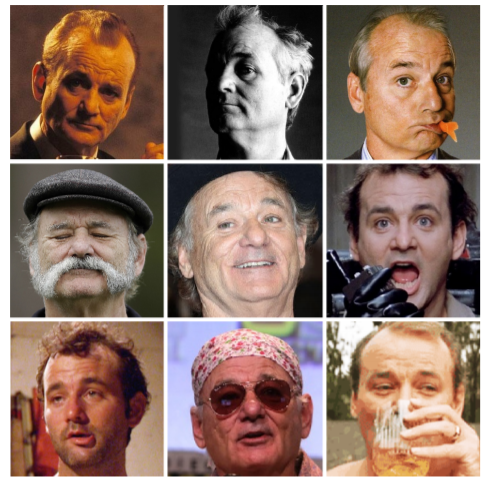
\includegraphics[scale=0.5]{img/the_same_person.png}
\caption{Very different pictures of a single individual}
\end{figure}


Facial recognition is an active area of research, spanning several disciplines such as image processing, pattern recognition, computer vision and neural networks. Engineering started to show interest in face recognition in the mid-1960’s. One of the pioneers in this topic was Woodrow W. Bledsoe. He developed a semi-automatic system that could classify photos of faces by hand using so-called a "RAND tablet" - a device that people could use to input horizontal and vertical coordinates on a grid using a stylus that emitted electromagnetic pulses. The system was used to record the coordinate locations of various facial features such as the eyes, nose, hairline or mouth. Gathered information were used by computers in further facial recognition. 


In 1988, Sirovich and Kirby applied the linear algebra to the problem of facial recognition, introducing the Eigenface approach. They showed that feature analysis on a collection of facial images could form a set of basic features. They were also able to show that less than one hundred values were required in order to accurately code a normalized face image. Few years later Turk and Pentland expanded the approach by discovering how to detect faces within images. This led to the first automatic face recognition. It was a real milestone in proving the feasibility of automatic facial recognition.

In the meantime another branch of study was being developed - the artificial neural networks. This, inspired by the human brain structure system turned out to be a breakthrough solution to many engineering problems. 

Nowadays, deep neural network approach is one of the most actively investigated method regarding the facial recognition problem. Deep Learning is at the cutting edge of what machines can do. It seems to provide the best results among all other facial recognition algorithms. 


%---------------------------------------------------------------------------




















\chapter{Face Recognition Process}

\section{Face Detection}
The process of recognizing a face in an image consists of two phases:

\begin{enumerate}
\itemsep0em
\item \textbf{Face detection} – detecting the pixels in the image which represent the face. 
\item \textbf{Face recognition} – the actual task of recognizing the face by analyzing the part of the image identified during the face detection phase.
\end{enumerate}

Numerous algorithms have been introduced and claimed to have accurate performance to tackle face detection problems. E.g. Principle Component Analysis, Local Binary Pattern, Fisherface algorithm, Gabor Wavelet method, Viola-Jones algorithm or the Artificial Neural Networks. In this work the Local Binary Pattern Algorithm (\textit{LBP})was used to extract the faces from the given image data set. LBP is not the most efficient algorithm among the others listed above, however it is good enough to gather the required amount of training data for the face recognition process, which is the main topic of this thesis. 

The problem of face detection is almost as complex as face recognition itself. The framework for both face detection and recognition is very similar, hence the difficulties that may be encountered are basically the same.
Faces have a wide variability in poses, shapes, sizes and texture. The problems or challenges in face detection and recognition are listed as follow:

\begin{itemize}
\itemsep0em
\item Illumination - the amount and type of light present during the image is captured can differ
\item Pose - a face varies depends on the position of the camera.
\item Presence of structural components such as moustache or beard
\item Facial expression 
\item Face occlusion such as glasses, scarf, mask etc.
\item Image quality 
\end{itemize}


\section{Face Recognition}
The face recognition phase can be applied in two different types of applications: 

\begin{enumerate}
\itemsep0em
\item Verification - the process of affirming that a claimed identity is correct by comparing the offered claims of identity with one or more previously enrolled templates. Verification systems are generally described as a 1-to-1 matching system because the algorithm tries to match the biometric presented by the individual against a specific biometric already present in the system.
\item Identification - the system attempts to determine the identity of an individual. The application  must check the biometric presented against all others already in the database. Identification systems are described as a 1-to-n matching system, where n is the total number of samples in the database. 
\end{enumerate}

Facial recognition can be approached by using many different kinds of machine learning algorithms. At a high level, these different algorithms can be classified into two groups based on the way they “learn” about data to make predictions: supervised and unsupervised learning.

The goal of both methods is to find a specific relationships or structure in the input data that allow us to effectively produce correct output data. The fundamental factor that differs those two algorithm groups is that the supervised algorithm is being "taught" from a given training data set, whereas an unsupervised algorithm is deriving the inherent structure of the data without using explicitly-provided labels. 

\subsection{Unsupervised learning}
\par
\textbf{Principal Component Analysis}
\\
The purpose of PCA is to reduce the large dimensionality of the data space to the smaller dimensionality of feature space, that nonetheless retains most of the sample's information. The method uses linear algebra to yield the directions (principal components) that maximize the variance of the data. 
\\
\par
\textbf{Self-organizing Map}
\\
Self-organizing map is a type of artificial neural network that belongs to a category of competitive learning networks. During training, the output unit that provides the highest activation to a given input sample is declared the winner and is moved closer to the input sample, whereas the rest of the neurons remain unchanged.

In short SOM algorithm implements a mapping from the high dimensional space to map units. Map units, so-called neurons, usually form a two-dimensional grid, therefore a SOM method provides a dimensionality reduction.
\\
\par
\textbf{Independent Component Analysis}
\\
Independent component analysis, as the name suggest, has a lot in common with Principal Component Analysis. Both PCA and ICA seek a set of basis vectors, that the inputs data is projected against. The difference between those two algorithms is that PCA finds the set of vectors that best explains the variability of the input data under the constraint that it is orthogonal to the preceding components, whereas in ICA each vector represents an independent component of the input data. 

\subsection{Supervised learning}
 
Nevertheless, nowadays the supervised machine learning is much more more common across a wide range of industry use cases. The most popular supervised algorithms in terms of facial recognition are briefly described below.
\\
\par
\textbf{Support Vector Machine}
\\
SVM belongs to the class of maximum margin classifiers. It performs a pattern recognition between two classes by finding a hyperplane that separates the largest possible fraction of points of the same class on the same side, while maximizing the distance from either class to the hyperplane. In terms of face recognition, the PCA is first used to extract features of face images and then discrimination functions between each pair of images are learned by support vector machine algorithm. 
\\
\par
\textbf{Artificial Neural Network}
\\
Artificial Neural Network is an approach, based on a large collection of neural units, so-called neurons, structurized in layers. The deep learning models are inspired by the way biological neural networks in the human brain process information. In case of face recognition we have to deal with the problem of processing very high-dimensional inputs. To face this problem the Convolutional Neural Network (\textit{CNN}) was introduced. 
\\\\
In this thesis we will take a closer look on Principal Component Analysis, Support Vector Machine and Artificial Neural Networks.
















\chapter{Principal Component Analysis}
\label{cha:PCA}

Principal Component Analysis is a statistical procedure that uses an orthogonal transformation to convert a set of observations of possibly correlated variables into a set of values of linearly uncorrelated variables called principal components. In fact this approach reduce number of feature vectors. The main advantages of the PCA are its low sensitivity to noise, the reduction of the requirements of the memory, and the increase in the efficiency due to the operation in a space of smaller dimensions. In face recognition problem PCA is based on extracting the characteristic features of the face and representing the face as a linear combination of the so called eigenfaces obtained from the feature extraction process. PCA for face recognition is usually called Eigenfaces method.


\section{Algorithm Background}

When using these sort of matrix techniques in computer vision, representation of images must be considered. A square, $N$ by  $N$ image can be expressed as an $N^{2}$ dimensional vector. 

\begin{equation}
X = ( x_{1}, x_{2}, ... , x_{N^{2}})
\end{equation}

where the rows of pixels in the image are placed one after the other. The values in the vector are the intensity values of the image - a single greyscale value. 

Say we have $M$ images in our training dataset containing $NxN$ pixels images. For each image we create an image vector as described above. Later on we built our database matrix representation.


\begin{equation}
ImagesMatrix = 
 \begin{pmatrix}
 ImageVector_{1} \\
 ImageVector_{2} \\
  \vdots  \\
 Image1vector_{M} 
 \end{pmatrix}
 \end{equation}
 
In the next step the average of the image set is calculated as:
\begin{equation}
averageFace = \frac{1}{M} \sum_{i=1}^{M} ImageVector_{i}
\end{equation}

The graphical representation of $avarageFace$ is presented in Figure 4.1.

\begin{figure}[H]
\centering
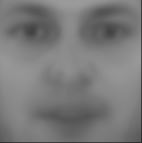
\includegraphics[scale=1]{avarage_face.jpg}
\caption{Avarage Face graphical representation}
\end{figure} 

$averageFace$ is calculated and subtracted from each face in the training set, which provides the set of normalized set of training images - matrix $A$. The normalization is computed as follows:

\begin{equation}
\phi_{i} = ImageVector_{i} - averageFace
\end{equation}

\begin{equation}
A = [\phi_{1}, \phi{2} \cdots \phi_{M}]
\end{equation}
 
In the next step the covariance matrix $C$ should be computed, from which the eigenvectors need to be derived. The basic formula for covariance matrix is presented in 4.6. 
 \begin{equation}
 C= AA^{T}
 \end{equation}
 
Since we know that dimension of matrix $A$ is $N^{2} x M$, we can derive the dimension of such a covariance matrix $C$: 

 \begin{equation}
 C \sim N^{2} x N^{2}
 \end{equation}

It turns out that using such a high-dimensional matrix $C$ would be highly inefficient for further calculations. As a result we would get $N^{2}$ eigenvectors. The solution to this problem is dimensionality reduction.

The matrix $C$ is computed as presented in 4.8

 \begin{equation}
 C= A^{T}A
\end{equation}

 \begin{equation}
 C \sim M x M
\end{equation}

The dimension of matrix C significantly decreased. In result of such an operation we will get $M$ eigenvectors each of $M$ dimension. 

\begin{equation}
Cv_{i} = \lambda_{i}v_{i}
\end{equation}

where $\lambda_{i}$ are eigenvalues and $v_{i}$ are eigenvectors. 

The next step is to choose the $K$ eigenvectors such as $K < M$ and the whole training set can be represented as a linear combination of those chosen vectors. The eigenvectors that corresponds to zeroes eigenvalues are discarded. 

The set of extracted significant eigenvectors have to be mapped back into the original dimensions, which provides the set of eigenfaces. 

Using linear algebra principles, we can perform the mapping as described in formula 4.11

\begin{equation}
u_{i} = Av_{i}
\end{equation}

\begin{equation}
||u_{i}|| = 1
\end{equation}

The eigenfaces $u_{i}$ may be considered as a set of features which characterize the global variation among face images. The graphical representation of eigenfaces can be seen below: 


\begin{figure}[H]
\centering
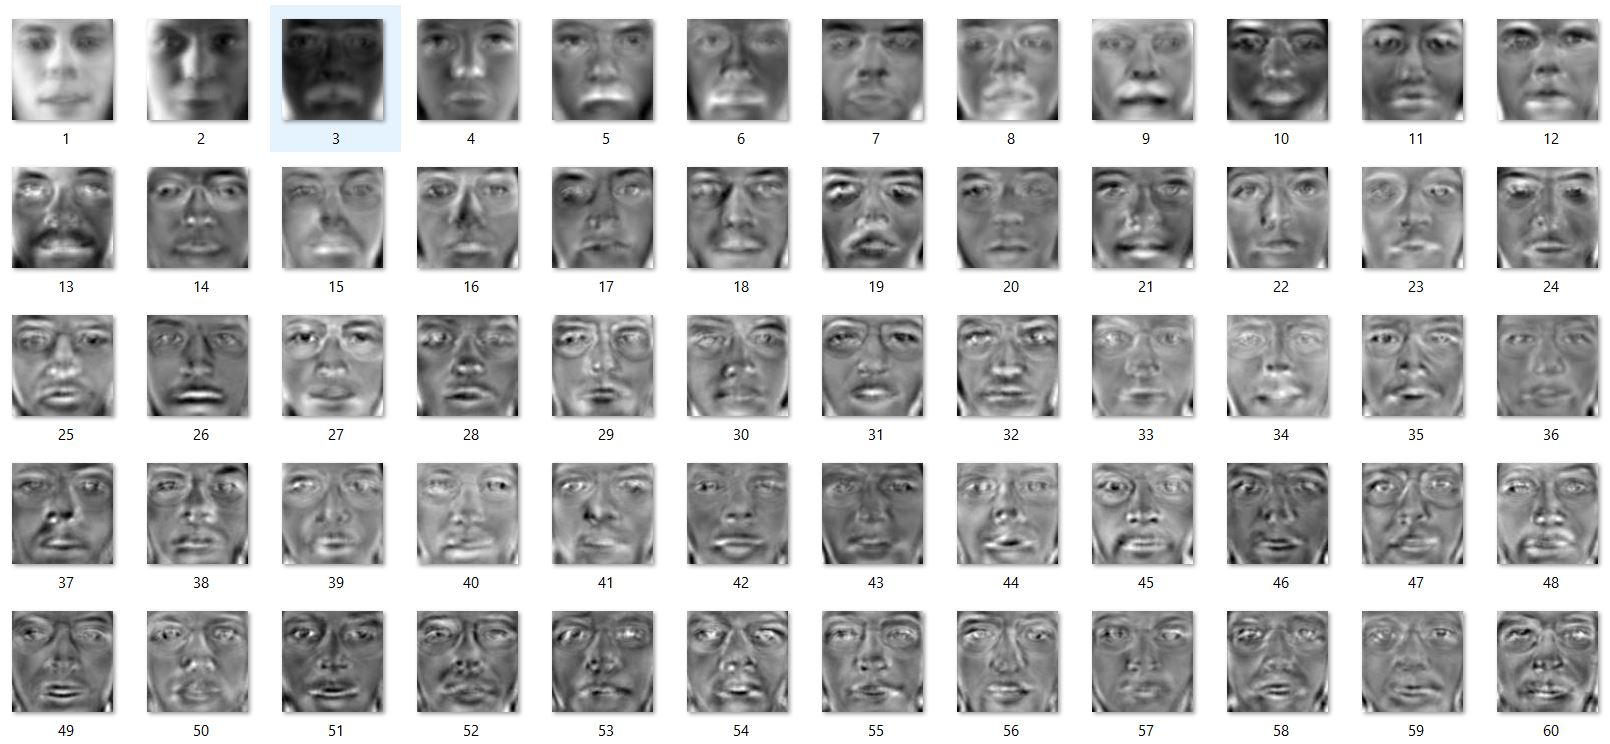
\includegraphics[scale=0.45]{eigenfaces.jpg}
\caption{Image representation of eigenfaces}
\end{figure}


\begin{figure}[H]
\centering
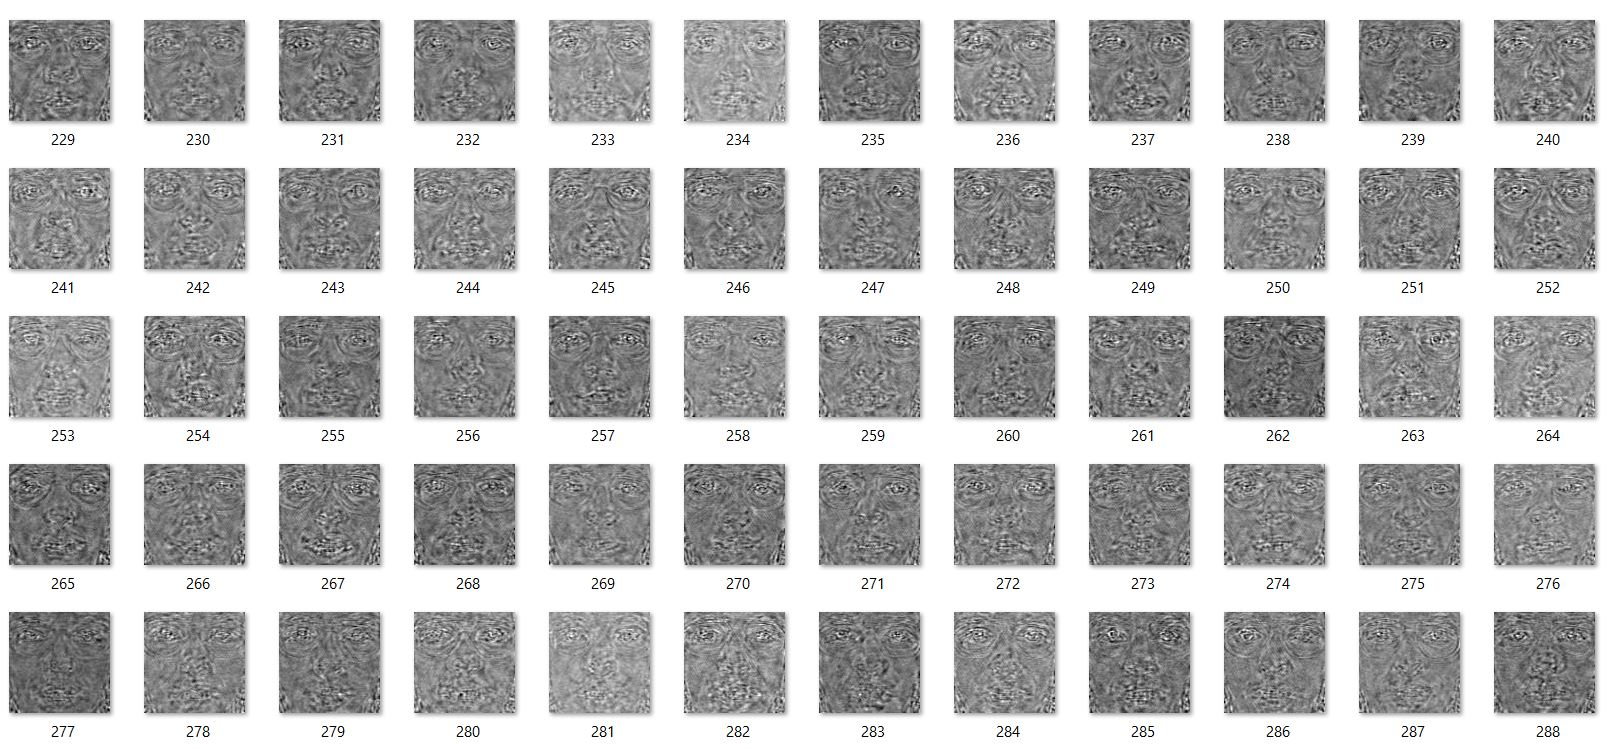
\includegraphics[scale=0.45]{eigenfaces_worse.jpg}
\caption{Less significant eigenfaces }
\end{figure}

On figure 4.2, we can observe 50 most significant eigenvectors - the ones with the highest eigenvalues, whereas figure 4.3 presents less significant eigenfaces. 

The next step is to represent each normalized face in a training set as a linear combination of previously extracted eigenfaces. In this way we can represent each face in a training set as a one dimensional vector with elements corresponding to each eigenface. 

\begin{equation}
\Omega_{i} =  \begin{pmatrix}
 w_{1} \\
 w_{2} \\
  \vdots  \\
 w_{K} 
 \end{pmatrix}
\end{equation}
 
The last step in the PCA algorithm is to project the unknown face  $x$ into space of eigenfaces as:

\begin{equation}
\Omega = U^{T} (x - averageFace) 
\end{equation}

where $U$ is the set of significant eigenvectors.

One simple way to determine to which face class $x$ belongs is minimizing the Euclidean distance 
\begin{equation}
\epsilon_{k} = ||\Omega - \Omega_{k}||
\end{equation}

where $\Omega_{k}$ is the weight vector representing the $k_{th}$ face class. The face $x$ is considered as belonging to class $k$ if the the minimum $\epsilon_{k}$ is smaller than some threshold $t$. Otherwise face $x$ is classified as unknown.

\section{Implementation and results}

The PCA - Eigenfaces algorithm was implemented with Python 3.6.1 with usage of numpy, scipy and PIL libraries. 

The performance of PCA based algorithm was evaluated with two image databases: Chicago Face Database (version 2.0.3) and Labeled Faces in the Wild Database (LFW).  The Chicago Face Database consists of good quality images with varying face expression and very similar capturing conditions for each sample. The Labeled Face in the Wild database contains images of peoples captured in various places, with various face expressions, light conditions, pose etc. The quality of images is rather poor. All the images in both the databases were converted to grey scale and normalized.


Samples from each database are presented below:

\begin{figure}[H]
\centering
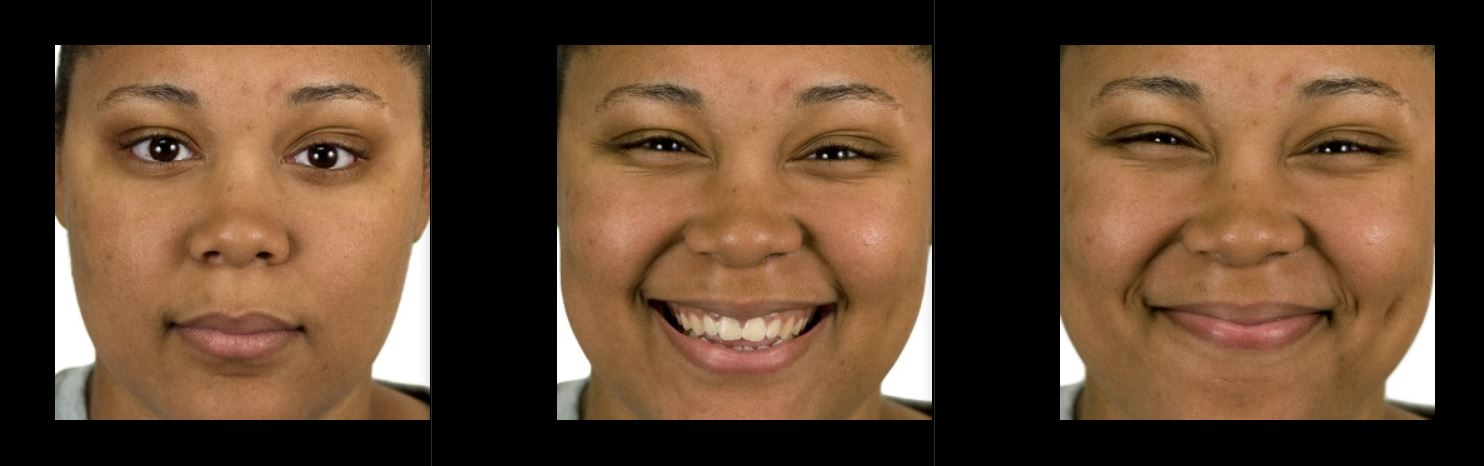
\includegraphics[scale=0.3]{CFD_samples.jpg}
\caption{Samples from Chicago Face Database}
\end{figure} 


\begin{figure}[H]
\centering
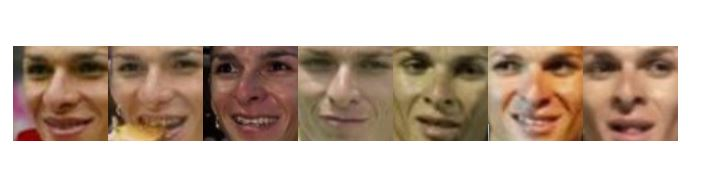
\includegraphics[scale=0.7]{lfw_samples.jpg}
\caption{Samples from Labeled faces in the Wild}
\end{figure} 

The first test was performed on 158 individuals from Chicago Face Database. Four out of the six images of a person were used for training and the remaining two were used to test the recognition rate. The choice of the training and testing images was made randomly.

Test was ran multiple times for different number of eigenfaces. The Figure 4.6 presents how the recognition rate depends on the amount of eigenfaces on which the tested image is projected. 

\begin{figure}[H]
\centering
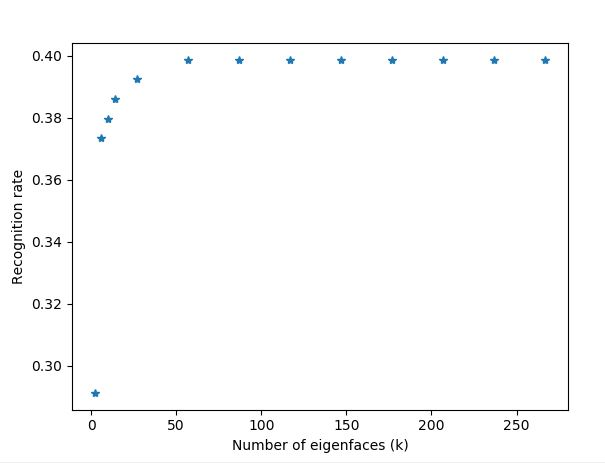
\includegraphics[scale=0.7]{rec_rate_vs_number_of_eigenfaces.jpg}
\caption{Recognition rate with varying number of eigenvectors}
\end{figure} 

The recognition rate stabilizes with $k = 54$ reaching the value of $0.3998$, which can be interpreted as the percentage of faces that were classified correctly. 

Figure 4.7 presents the image representation of three chosen eigenfaces from CFD database.

\begin{figure}[H]
\centering
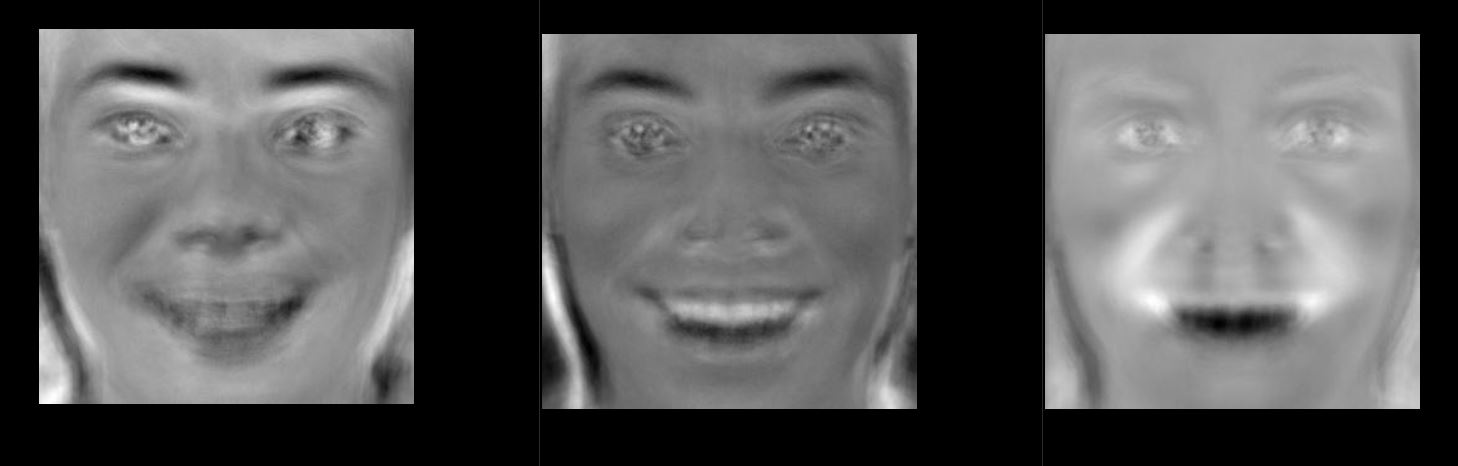
\includegraphics[scale=0.3]{eigenfaces_CFD.jpg}
\caption{CFD eigenfaces}
\end{figure} 


The second test was performed on the set of 40 individuals from Labeled faces in the Wild database. 27 out of 30 images of a person were used for training and the remaining 3 were used to test the recognition rate. The choice of the training and testing images was made randomly.
The PCA algorithm achieved $12,22\%$ of accuracy. The result is poor, as expected. The quality of images is by far not good enough, to successfully perform the PCA algorithm.




\chapter{Artificial Neural Networks}

One of the most powerful methods to solve the face recognition problem are Artificial Neural Networks. 
A good definition of ANN, is given by Haykin [TODO] describing ANN as a parallel combination of simple  processing unit which can acquire knowledge from environment through a learning process and store the knowledge in its connections. The idea of Artificial Neural Network was inspired by biological neural networks (in particular the brain). 

\section{Biological background}
A neuron, in a biological sense, is a cell that carries and processes information - electric signal. The typical neuron is composed of cell body (perikarion) and two types of "branches": axons and dendrites. The cell body consists of plasma and a nucleus that holds information about hereditary traits. Each neuron receives an information from other neurons through the dendrites and transmits the processed information via axons. Axon - dendrites connection is called synapse. 

\begin{figure}[H]
\centering
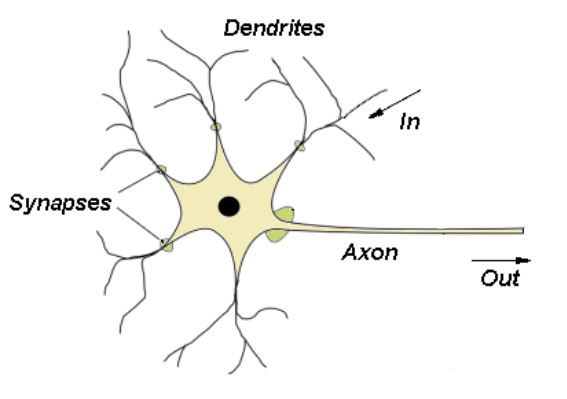
\includegraphics[scale=1]{neuron_schema.jpg}
\caption{Biological Neuron Schema}
\end{figure} 

The synapse's effectiveness can be adjusted by the signals passing through it so that the synapses can learn from the activities in which they participate. 

A typical person is capable of making complex perceptual decisions such as face recognition within a few hundred milliseconds. These decisions are made by a network of neurons whose operational speed is only a few milliseconds. This implies that the computations cannot take more than about 100 serial steps. This is knows as a hundred step rule: the brain runs parallel programs that are at most 100 steps long for such a tasks.

It can be deduced that the amount of information sent from one neuron to another is very small. Hence, the critical information is not transmitted directly, but captured and distributed in the neuron interconnections. 

That is also one of the features of Artificial Neural Networks. The system inspired by human brain are also hoped to posses some of the most desired brain's characteristics such as:

\begin{itemize}
\itemsep0em 
\item massive parallelism 
\item distributed representation and computation
\item learning ability 
\item adaptability
\item fault tolerance
\end{itemize}


\section{Artificial Neural Network architecture}

\subsection{Forward pass}

The smallest unit of computation in a neural network is the neuron, also called a node or unit. It receives an input from the other neurons or (in case of input neurons) from the external source. Each input has an associated weight, which is assigned proportionally to its relative importance to other inputs. The neuron produces the output by applying so called activation function to the weighted sum of its inputs.

\begin{figure}[H]
\centering
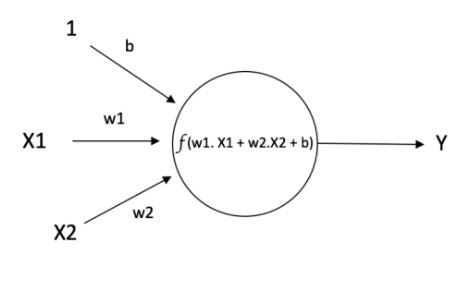
\includegraphics[scale=0.65]{single_neuron.jpg}
\caption{Single Neuron}
\end{figure} 


The activation function is applied in order to introduce non-linearity into the neurons' output. The choice of activation function is wide and it remains as an active area of research. The most commonly used activation functions are presented below: 

\begin{itemize}
\itemsep0em 
\item Sigmoid: squashes the input into the range between 0 and 1 
\begin{equation}
\sigma (x) = \frac{1}{1+\exp(-x)} 
\end{equation}
\item Hyperbolic tangent: squashes the input into the range between -1 and 1
\begin{equation}
tanh(x) = \frac{e^{x} - e^{-x}}{e^{x} + e^{-x}}
\end{equation}
\item Rectified Linear Unit (ReLU): It takes a real-valued input and thresholds it at zero
\begin{equation}
f(x) = max(0, x)
\end{equation}
\end{itemize}

According to the recent publications the ReLU function is believed to perform better than the other activation functions. Its simplicity reduces the computational complexity - it does not involve expensive operations such as exponentials. Another big advantage of ReLU is non-saturation of its gradient, which greatly accelerates the convergence of stochastic gradient descent compared to the sigmoid / tanh functions (TODO paper by Krizhevsky et 
al).

The general equation describing the neural network forward pass is given by:

\begin{equation}
\vec{o} = f(\vec{w} \cdot \vec{x} + b) 
\end{equation}

where $o$ is the output vector, $f$ is an activation function, $\vec{w}$ is a weights vector, $\vec{x}$ is a vector of layer input, $b$ is a bias.

\section{Backpropagation}

One of the main requirements for training this kind of algorithms is data. All learning algorithms use data in their training processes, but ANN require more than most.Given the data, there are various learning algorithms, from which gradient descent (backpropagation) is considered the most successful of all of them.


Backpropagation, also called gradient descent, is a common method for training a neural network. It is used for training Multilayer Perception Network as well as Convolutional Neural Network.

The basic idea of gradient descent method is to adjust the parameters of the neural networks in the way that the computed difference between predicted and expected values will be minimized. 

The choice of error functions (cost functions) is wide. One of the simplest approaches is to calculate the Euclidean distance between the predicted $o$ and expected $o'$ values: 

\begin{equation}
E_{1}(o,o') = \frac{||o-o'||^{2}}{2}
\end{equation}

The error can be also calculated using Mean Squared Error: 
\begin{equation}
E_{2}(o,o') = \frac{\sum_{k=1}^{K}(o_{i} - o'_{i})^2}{K}
\end{equation}
where $K$ is the size of output vector.

When using a neural network to perform classification and prediction, it is usually better to use cross-entropy error than classification error or mean squared error, due to the better convergence of the gradient.

The cross-entropy error function for multi-class output is defined as:

\begin{equation}
E_{3}(o, o') = -\sum_{i=1}^K o'_{i} \ln(o_{i})\end{equation} 


Since the goal of backpropagation is to minimize the error E, which depends on the network weights, we have to deal with all weights in the network one at a time.
To perform the backpropagation, the output of each unit from the forward pass must be stored. The gradients with respect to each parameter $w_{ij}$ is being calculated.

\begin{enumerate}
\itemsep0em
\item As a first step we calculate so-called errors $\delta_{i}^{(o)}$ for the output units:

\begin{equation}
\delta_{i}^{(o)} = \frac{\partial E}{\partial o_{i}} f'(z_{i})
\end{equation}

where $z_{i}$ is the input to the output layer.
\item We determine $\delta_{i}^{(l)}$ for all hidden layers in the network:

\begin{equation}
\delta_{i}^{(l)} = f'(z_{i}^{(l)}) \sum_{k=1}^{m^{(l+1)}} w_{i,k}^{(l+1)} \delta_{k}^{(l+1)}
\end{equation}
where $m^{(l)}$ is the number of units in layer $l$.
\item We calculate the derivative:
\begin{equation}
\frac{\partial E}{\partial w_{j,i}^{(l)}} = \delta_{j}^{(l)}y_{i}^{(l-1)}
\end{equation}
\item Once all partial derivatives have been computed, the gradient descent is performed by subtracting from each weight the increment:
\begin{equation}
\Delta w_{ij} = \lambda z_{j}^{(l-1)} \delta_{j}^{(l)}
\end{equation}

where $\lambda$ is a learning rate, which determines how fast the network coefficients change. 
\end{enumerate}

After choosing the initial weights of the network randomly, the backpropagation algorithm is used to compute the necessary corrections. The neural network training process can be decomposed in the following steps:

\begin{enumerate}
\itemsep0em 
\item Feed-forward pass
\item Backpropagation of each layer
\item Weight updates
\end{enumerate}
The algorithm is stopped when the value of the error function is sufficiently small.


\subsection{ANN topology}

The architecture of an artificial neural network defines how its several neurons are arranged, or placed, in relation to each other. In general an artificial neural network architecture can be divided into three parts (figure 6.2):

\begin{enumerate}
\itemsep0em 
\item Input layer - responsible for receiving normalized information, signals, features, or measurements from the user.
\item Hidden layer (or layers) - responsible for further information processing such as extracting patterns associated with the process. 
\item Output layer - responsible for producing and presenting the final network outputs, which result from the previous information processing.
\end{enumerate}

\begin{figure}[H]
\centering
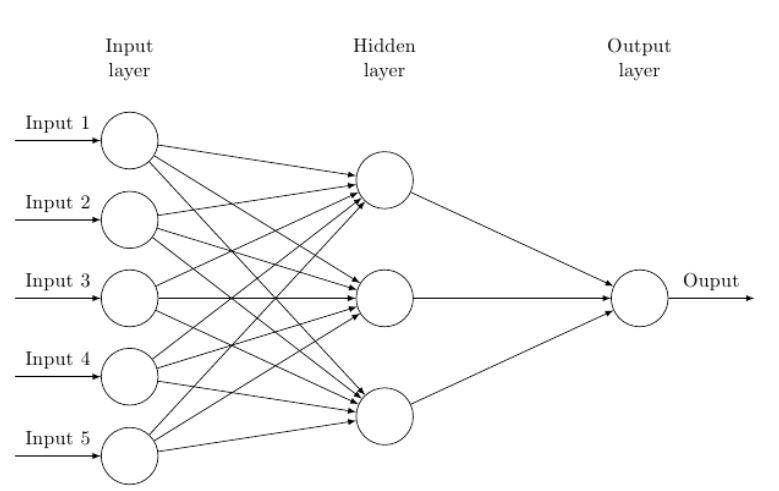
\includegraphics[scale=0.65]{ANN_schema.jpg}
\caption{Basic Artificial Neural Network Schema}
\end{figure} 

The presented ANN structure performs a feed-forward process. The connections only project forward, that is, neurons in a layer send the signal only to the subsequent layer. Furthermore, there are no connections between neurons in the same layer or between non-adjacent layers. 

There are plenty various configurations of feed-forward ANN, which can differ in the number of neurons in each layer as well as in the amount of layers. 

\begin{figure}[H]
\centering
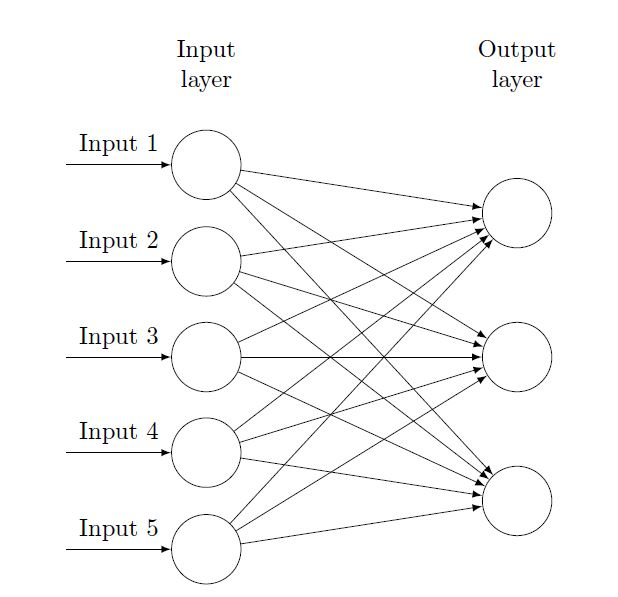
\includegraphics[scale=0.65]{single_ANN_schema.jpg}
\caption{Single-layer Artificial Neural Network Schema}
\end{figure} 

\begin{figure}[H]
\centering
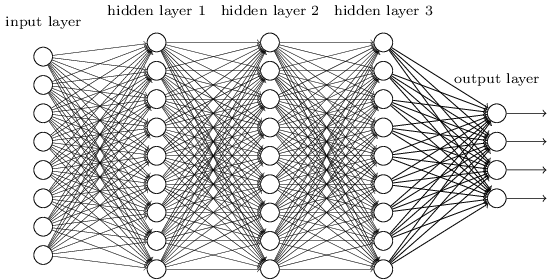
\includegraphics[scale=0.65]{img/neural_net.png}
\caption{Example of Deep Neural Network architecture}
\end{figure}

The neural network with more than one hidden layer is known as Deep Neural Network. (Figure 6.4). This type of ANN is suitable for processing very high-dimensional data, hence it seems to be a good choice for the facial recognition system design. 




\chapter{Multi Layer Perception}

The multi layer perception is the most known and most frequently used type of neural network. It consists of at least three layers. The difference between Multi and Single layer perception is that, the first one can learn non-linear functions, whereas the second one is only suitable for solving linear problems. 

Multilayer perceptrons are often applied to supervised learning problems: they are being trained on a set of input-output pairs and learn to model the dependencies between the given inputs and outputs. Training, so-called backpropagation, involves adjusting the parameters of the model in order to minimize the error. MLP performs well with relatively low dimensional inputs. 


\section{Implementation and test result}
Due to the big amount of parameters its rather a poor solution for working with the images as its inputs. To proceed with MLP algorithm we need relatively low dimensional data. The idea to implement Face Recognition system using MLP is to connect Multi Layer Perception model with Principal Component Analysis algorithm. 

The first step in this approach is to perform PCA on every image in a training data set. PCA produces a weight vector, (4.13) for an image, hence we can represent each image in a low dimensional space. The dimension depends on the number of eigenvectors chosen for Principal Component Analysis algorithm. 

\begin{equation}
X =
\left[
\begin{matrix}
w_{11} & w_{21} & \cdots & \cdots & w_{m1}\\
w_{12} & w_{22} & \cdots & \cdots & w_{m2}\\
w_{13} & w_{23} & \cdots & \cdots & w_{m3}\\
w_{14} & w_{24} & \cdots & \cdots & w_{m4}\\
\cdots & \cdots & \cdots & \cdots & \cdots\\
\cdots & \cdots & \cdots & \cdots & \cdots\\
w_{1k} & w_{2k} & \cdots & \cdots & w_{mk}
\end{matrix}
\right]
\end{equation}

where $k$ is a number of eigenvectors and $m$ is amount of data in a training data set.

Since the MLP is a supervised algorithm, to train the model the data labels are required. Each label was represented as a k-dimensional vector.

\begin{equation}
Y =
\left[
\begin{matrix}
0 & 1 & \cdots & \cdots & 0\\
0 & 0 & \cdots & \cdots & 0\\
0 & 0 & \cdots & \cdots & 1\\
1 & 0 & \cdots & \cdots & 0\\
\cdots & \cdots & \cdots & \cdots & \cdots\\
\cdots & \cdots & \cdots & \cdots & \cdots\\
0 & 0 & \cdots & \cdots & 0
\end{matrix}
\right]
\end{equation}

The goal is to train the model in a way that given the matrix $X$ MLP will produce close approximation of matrix $Y$. 

For training the model backpropagation algorithm was used. 
\\
\begin{python}
def back_prop(epochs, X, Y, Wh, Wp, activation, l_rate):
    for i in range(epochs):
        H = activation(np.dot(X, Wh))  
        Z = activation(np.dot(H, Wp)) 
        E = error(Y, P)
        dP = E * activation(Z, deriv=True) 
        dH = dP.dot(Wp.T) * activation(H, deriv = True)  
        Wz += l_rate * H.T.dot(dP)  
        Wh += l_rate * X.T.dot(dH)  
        if i % 10000 == 0:
            per = check_performance(Z)
            if per > 0.98:
                break
\end{python}


The neural network performance varies depending on the change of various parameters such as:

\begin{itemize}
\itemsep0em 
\item amount of input data
\item amount of neurons in hidden layers
\item initial weights
\item activation function
\item learning parameter
\end{itemize}

The tests were performed on two different databases: 
\begin{itemize}
\itemsep0em 
\item Chicago Face Database - pictures captured in controlled environment
\item Labeled Faces in Wild database - pictures captured in uncontrolled environment, with various lightning conditions, pose, facial expression etc. 
\end{itemize}


\section{Tests on pictures captured in controlled environment}

The database was divided into training and testing samples. The training was performed using 3 pictures of the individual, one pictures was used to test the trained model. 

\begin{figure}[H]
\centering
\begin{subfigure}[b]{.2\linewidth}
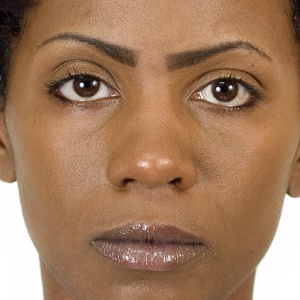
\includegraphics[width=\linewidth]{img/CFD1.jpg}
\end{subfigure}
\centering
\begin{subfigure}[b]{.2\linewidth}
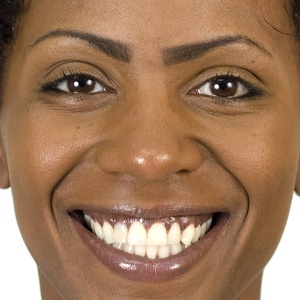
\includegraphics[width=\linewidth]{img/CFD2.jpg}
\end{subfigure}
\centering
\begin{subfigure}[b]{.2\linewidth}
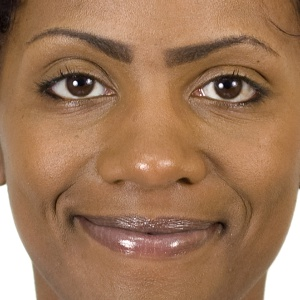
\includegraphics[width=\linewidth]{img/CFD3.jpg}
\end{subfigure}
\caption{Examples of one person pictures in the training dataset}
\end{figure}


\begin{figure}[H]
\centering
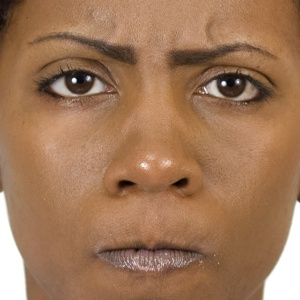
\includegraphics[scale=0.3]{img/CFD4.jpg}
\caption{Testing image}
\end{figure} 


The tests were performed using MLP topology presented on figure 7.1 (???).

\begin{figure}[!h]
\centering
\begin{tikzpicture}[
           > = Stealth, semithick,
plain/.style = {draw=none, fill=none, yshift=11mm,
                text width=7ex,  align=center},% for text in images, 
   ec/.style = {draw=none},% for emty cells
  net/.style = {% for matrix style
    matrix of nodes,
    nodes={circle, draw, semithick, minimum size=12mm, inner sep=0mm},% circles in image
    nodes in empty cells,% for not used cells in matrix
  column sep = 16mm, % distance between columns in matrix 
     row sep = -3mm  % distance between rows in matrix
            },
]
\matrix[net] (m)% m is matrix name, it is used for names of cell: firs has name m-1-1
                % in empty space between ampersands will show circles: 
                % i.e.: nodes of the neural network
{
|[plain]| $Input$ & |[plain]| $Hidden$ & |[plain]| $Output$ \\
|[ec]|                &                         & |[ec]|                  \\
                      & |[ec]|                  & |[ec]|                  \\
|[ec]|                &                         &                         \\
                      & |[ec]|                  & |[ec]|                  \\
|[ec]|                &                         &                         \\
                      & |[ec]|                  & |[ec]|                  \\
|[ec]|                &                         & |[ec]|                  \\
};
\% inputs
\foreach \in [count=\ir from 1] in {3,5,7}
\draw[<-] (m-\in-1.west) -- node[above]{}+(-12mm,0);
% connections between nodes in the first and second layer
\foreach \j in {3,5,7}
{
\foreach \k in {2,4,6,8} \draw[->] (m-\j-1) -- (m-\k-2);
}
% connections between nodes in the second and third layer
\foreach \j in {2,4,6,8}
{
\foreach \k in {4,6} \draw[->] (m-\j-2) -- (m-\k-3);
}
% output
\draw[->] (m-4-3.east) -- node[above] {} +(12mm,0);
\draw[->] (m-6-3.east) -- node[above] {} +(12mm,0);
    \end{tikzpicture}
\caption{Neural Network with one hidden layer}
\end{figure}


\subsection{20 individuals}

The first step is to set a number of eigenvectors that the image will be represented with. We do it using previously implemented PCA algorithm. 

\begin{figure}[H]
\centering
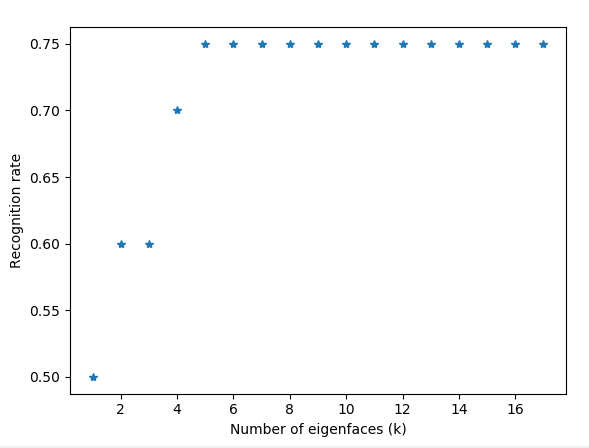
\includegraphics[scale=0.7]{img/tests/20ppl/PCA_on_20ppl_vs_k.png}
\caption{Recognition rate with varying number of eigenvectors for 20 individuals}
\end{figure} 

From this results, we can conclude that $k = 6$ is the sufficient amount of eigenvectors to properly represent each sample image. 

Test was performed on a data set with 20 individuals.
The PCA-MLP algorithm was ran with following parameters:

\begin{itemize}
\itemsep0em 
\item number of hidden layers = 1
\item number of neurons in hidden layers = 10
\item initial weights chosen randomly in a range [0:1]
\item sigmoid activation function
\item learning parameter = 1
\item number of eigenvectors $k = 6$
\end{itemize}

In order to examine accuracy of PCA-MLP algorithm we check if the index of obtained outputs' maximum value is equal to the index of maximum value of desired output. The accuracy is a value representing percentage of pictures that fulfills this requirement.

As the first step the influence of a learning rate parameter was examined.\\
\textbf{Learning rate = 1}\\
\begin{figure}[H]
\centering
\begin{subfigure}[b]{.45\linewidth}
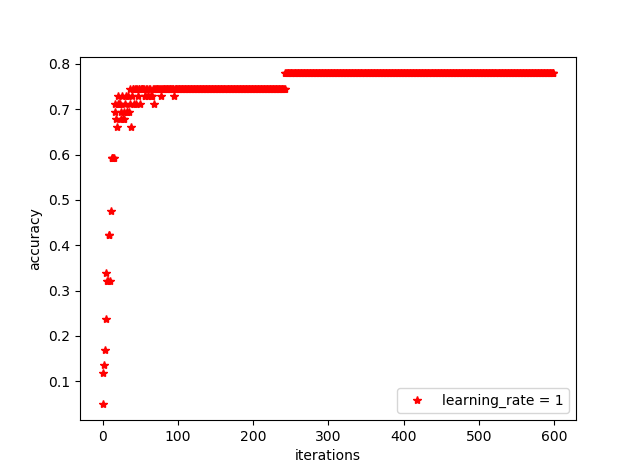
\includegraphics[width=\linewidth]{img/tests/20ppl/learnig_rate1_v1.png}
\end{subfigure}

\begin{subfigure}[b]{.45\linewidth}
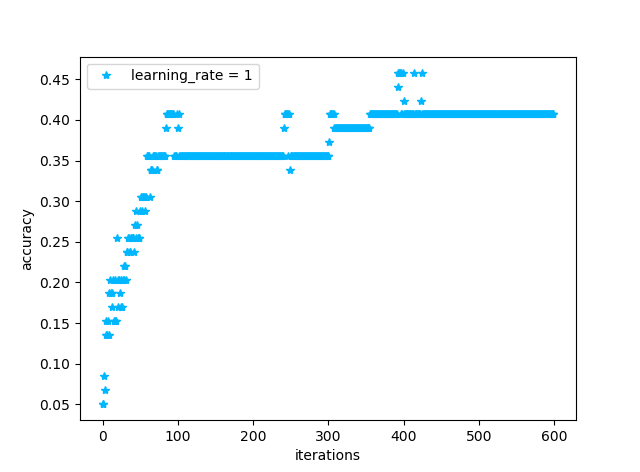
\includegraphics[width=\linewidth]{img/tests/20ppl/learnig_rate1_v2.png}
\end{subfigure}
\begin{subfigure}[b]{.45\linewidth}
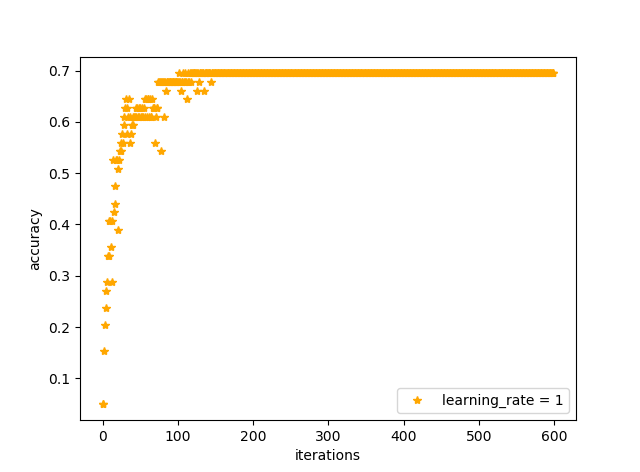
\includegraphics[width=\linewidth]{img/tests/20ppl/learnig_rate1_v3.png}
\end{subfigure}
\caption{Learning rate = 1, initial weights chosen randomly}
\label{fig:animals}
\end{figure}

The neural network with learning rate = 1 is very unstable and strongly depends on initial weights. 

The tests were performed for different learning rate values:

\begin{figure}[H]
\centering
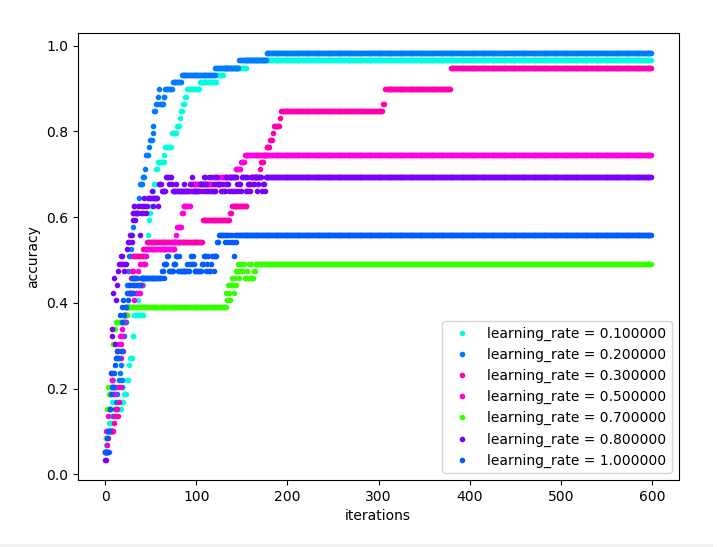
\includegraphics[scale=0.7]{img/tests/20ppl/learning_rates.png}
\caption{Algorithm accuracy with different learning rates}
\end{figure}

The learning rate is one of the most important hyper-parameters to tune for training neural networks. If the learning rate is low, then training is more reliable, but optimization will take more time because the weights changes are tiny.

For each experiment approximately 400 iterations were enough to sufficiently train the network.
 
To compare the accuracy of PCA algorithm itself with connection of PCA and MLP algorithms, the PCA results should be examined. The highest obtained recognition rate ( figure 7.4)  is 0.75.

The testing phase was made using the model that was train with following parameters:

\begin{itemize}
\itemsep0em
\item number of hidden layers = 1
\item number of neurons in hidden layers = 10
\item initial weights chosen randomly in a range [0:1]
\item sigmoid activation function
\item learning parameter = 0.2
\item number of eigenvectors $k = 6$
\end{itemize}


Obtained results are good. 18 out of 20 people were recognized correctly - the recognition rate reached 90\%, which is 15 percentage points better than result of PCA algorithm.


\subsection{40 individuals}

The choice of a number of eigenvectors representing the images in a small database is straightforward as presented in section (???). 

Following the same procedure as in section (???) we can derive the optimal (for PCA algorithm) $k$ value. 

\begin{figure}[H]
\centering
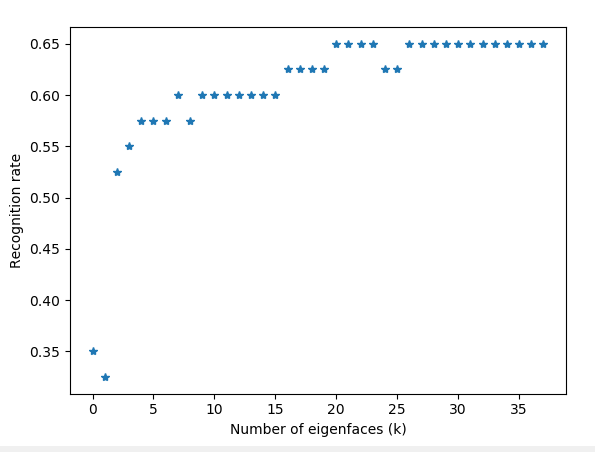
\includegraphics[scale=0.5]{img/tests/40ppl/PCA_40.png}
\caption{Recognition rate with varying number of eigenvectors for 40 individuals}
\end{figure} 

When dealing with a bigger database, we have to find a balance between a sufficient amount of eigenfaces to represent an image and an amount of data that can be applied as the input of multilayer perception network, so that we'll obtain acceptable training result in a reasonable time. The bigger input dimension, the harder it is to train the network. 

In this case input dimension = 27 is still low enough to be processed with MLP network, hence parameter $k$ was set to 27.

Test was performed with following parameters:

\begin{itemize}
\itemsep0em
\item dimension of input data = 27
\item number of hidden layers = 1
\item number of neurons in hidden layers = 27
\item initial weights chosen randomly in a range [0:1]
\item sigmoid activation function
\item learning rate = 0.2
\end{itemize}

The result of training algorithm. 

\begin{figure}[H]
\centering
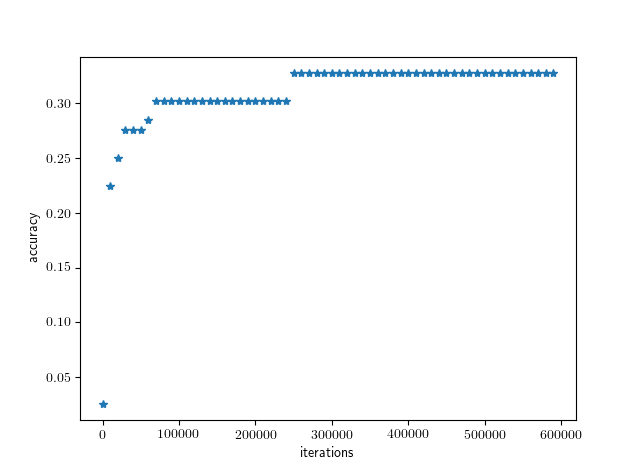
\includegraphics[scale=0.5]{img/tests/40ppl/k=27,h=27,60000epoch/res.png}
\caption{number of eigenvectors = 27, number of hidden neurons = 27}
\end{figure} 

The execution of the algorithm took 4 min 54 sek. The results are not satisfying.  

The next interesting parameter in terms of neural network performance is a number of neurons in a hidden layer. This topic is still an active area of research, and the major answers are driven by tests and experience. In the previous experiment, amount of hidden neurons was equal to the amount of input neurons and it does not seem to be a good solution. The recognition rate in the network trained as such reached 22,5\%, which is rather poor. The next step is to check if increasing or decreasing the amount of neurons in a hidden layer will help to improve the network performance. 

Using too few neurons in the hidden layers will result in underfitting. Underfitting occurs when there are too few neurons in the hidden layer to adequately detect the signals in a complicated data set.

On the other hand too many neurons in the hidden layer can result in several problems.
First of all overfitting - occurs when the neural network has so much information processing capacity that the limited amount of information contained in the training set is not enough to train all of the neurons in the hidden layers. Second of all, there is another problem that can be encountered even if the training data is sufficient. A large number of neurons in the hidden layer can increase the time it takes to train the network. The proper compromise must be reached between too many and too few neurons in the hidden layer.

There are several rule-of-thumb methods for determining an sufficient number of neurons in the hidden layers, such as the following:

\begin{itemize}
\itemsep0em 
\item The number of hidden neurons should be between the size of the input layer and the size of the output layer.
\item The number of hidden neurons should be 2/3 the size of the input layer, plus the size of the output layer.
\item The number of hidden neurons should be less than twice the size of the input layer.
\end{itemize}

In our case we have 27 input neurons and 40 output neurons. According to the listed rules we have 3 possibilities:

\begin{enumerate}
\itemsep0em 
\item the amount of hidden neurons should be in range between $27$ and $40$. 
\item the amount of hidden neurons should be equal to $0.6 * 27 + 40 \sim 56$
\item the amount of hidden neurons should be less than $\frac{27}{2} = 13.5$
\end{enumerate}

Each of the possibilities was examined. The results not only differ in the accuracy of the algorithm but also in the execution time. 

\begin{figure}[H]
\centering
\begin{subfigure}[b]{.45\linewidth}
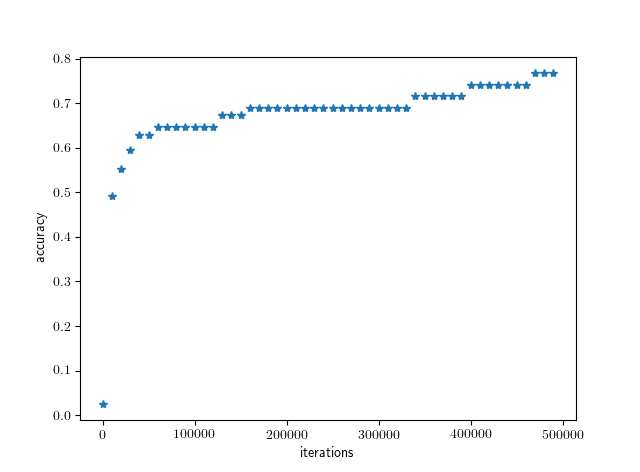
\includegraphics[width=\linewidth]{img/tests/40ppl/k=27,h=10,50000epoch/res.png}
\caption{10 hidden layers}
\end{subfigure}

\begin{subfigure}[b]{.45\linewidth}
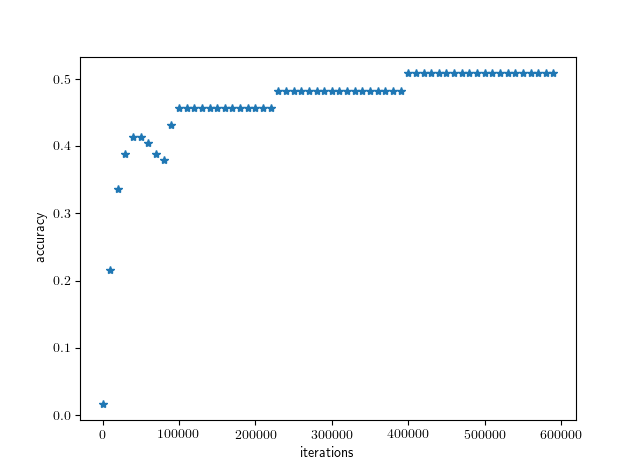
\includegraphics[width=\linewidth]{img/tests/40ppl/k=27,h=33,60000epoch/res.png}
\caption{33 hidden layers}
\end{subfigure}
\begin{subfigure}[b]{.45\linewidth}
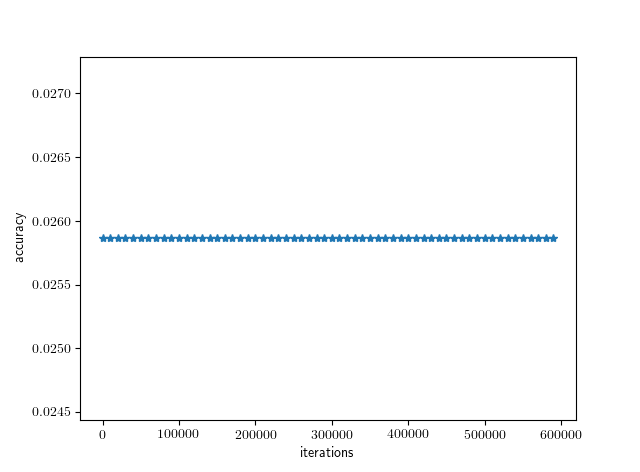
\includegraphics[width=\linewidth]{img/tests/40ppl/k=27,h=56,60000epoch/res.png}
\caption{56 hidden layers}
\end{subfigure}
\caption{Training accuracy for different amount of hidden neurons}
\end{figure}

\begin{center}
    \begin{tabular}{ | l | l | l | p{5cm} |}
    \hline
    Number of hidden neurons &  $10$ & $33$ & $56$ \\ \hline
    Execution time[sek] &  $114$  & $173$ & $216$ \\ \hline
	Recognition Rate & $70\%$ & $43.5\%$ & $2.5\%$ \\ \hline
    Training accuracy & $76.5\%$ & $50\%$ & $2.5\%$\\
    \hline
    \end{tabular}
\end{center}

The best results were achieved with 10 hidden layers. Comparing these results with the result of PCA algorithm on the same data, it seems that the performance of both is very similar. The reason for that might be not sufficient amount of training data. There is a technique that is facing this problem - so-called data augmentation.

It is a widely used method in many machine learning tasks to enlarge the training data set size and avoid overfitting. The goal of this process is to create new samples from the original training data by, for example, flipping, distorting, adding a small amount of noise to, or cropping a patch from an original image.

The first transformation is shifting  the image in four directions - left, right, down, up.


\begin{figure}[H]
\centering
\begin{subfigure}[b]{.3\linewidth}
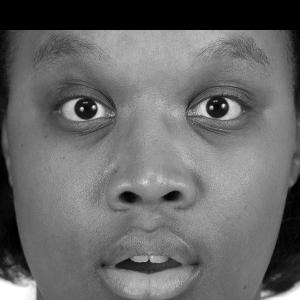
\includegraphics[width=\linewidth]{img/tests/shifts/shifted_image0.jpg}
\end{subfigure}
\centering
\begin{subfigure}[b]{.3\linewidth}
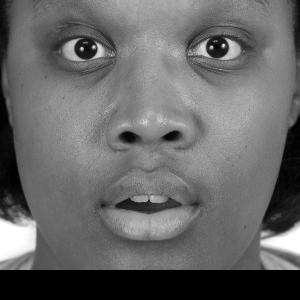
\includegraphics[width=\linewidth]{img/tests/shifts/shifted_image1.jpg}
\end{subfigure}


\begin{subfigure}[b]{.3\linewidth}
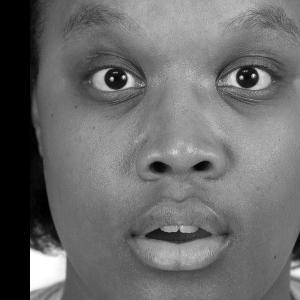
\includegraphics[width=\linewidth]{img/tests/shifts/shifted_image2.jpg}
\end{subfigure}
\begin{subfigure}[b]{.3\linewidth}
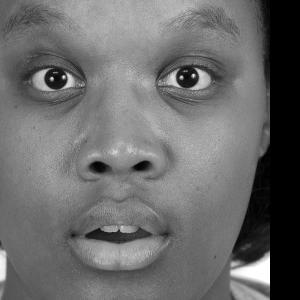
\includegraphics[width=\linewidth]{img/tests/shifts/shifted_image3.jpg}
\end{subfigure}
\caption{Shift transformations}
\end{figure}

Another applied image transformation is flipping the content of the image from left to right.

\begin{figure}[H]
\centering
\begin{subfigure}[b]{.3\linewidth}
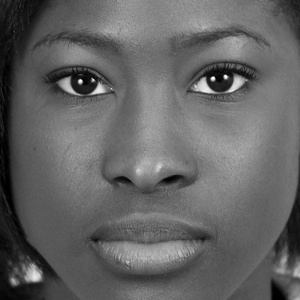
\includegraphics[width=\linewidth]{img/tests/shifts/image.jpg}
\end{subfigure}
\centering
\begin{subfigure}[b]{.3\linewidth}
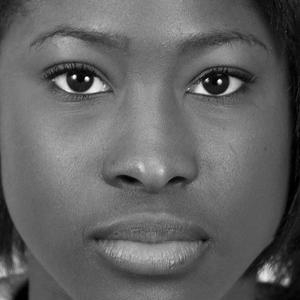
\includegraphics[width=\linewidth]{img/tests/shifts/flipped_image.jpg}
\end{subfigure}
\caption{Flipping transformation}
\end{figure}

Increasing amount of training data makes the training process much longer. It took about 15 min to train the network. In our case the results did not improve, but this is mainly because the training data is not varied in terms of shifting. The face is always in the same position in the picture. 
The recognition rate was 42,5\%, which is much worse, then before enlarging the data set. 
 
The algorithm was tested with Chicago Face Database, where all the individuals were captures in controlled environment. 
The samples of each individual differs only in terms of face expression. It is much more challenging to build a system that is not sensitive for changing the light conditions, the picture quality, face pose and many other factors. 

\section{Tests on pictures captured in uncontrolled environment}

To test the algorithm the Labeled Faces in Wild database was used. The quality of images is much worse then in the previous examples, so the tests result are expected to be worse. 


\begin{figure}[H]
\centering
\begin{subfigure}[b]{.2\linewidth}
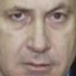
\includegraphics[width=\linewidth]{img/tests/lwf/sample1.jpg}
\end{subfigure}
\centering
\begin{subfigure}[b]{.2\linewidth}

\includegraphics[width=\linewidth]{img/tests/lwf/sample2.jpg}
\end{subfigure}
\caption{Exemplary samples from LFW database}
\end{figure}

Test was performed on 20 individuals with 30 pictures each. The training set for each person consists of 27 samples, 3 pictures were used to test the model. 

\subsection{One hidden layer}

The tests were performed in the same topology as presented in figure(??)

As in the previous examples PCA was performed as a first step. The results (figure 7.13) are very poor as expected. 

\begin{figure}[H]
\centering
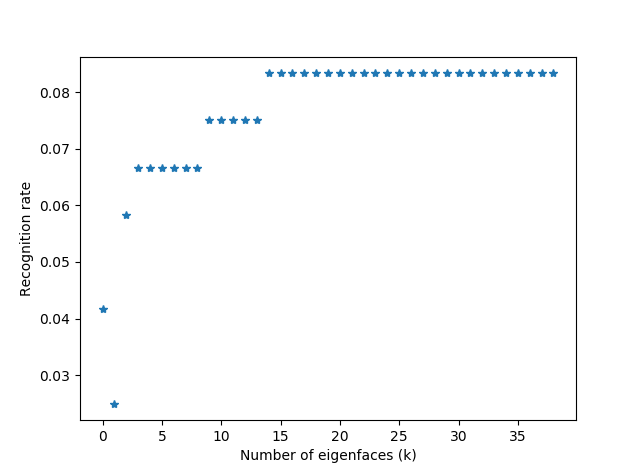
\includegraphics[scale=0.5]{img/tests/lwf/40ppl/PCA.png}
\caption{Recognition rate with varying number of eigenvectors for 20 individuals}
\end{figure} 

The question is how much can we improve our results with applying MLP network.


Model was trained with with following parameters:

\begin{itemize}
\itemsep0em
\item number of hidden layers = 1
\item initial weights chosen randomly in a range [0:1]
\item sigmoid activation function
\item learning parameter = 0.2
\end{itemize}

and various dimension of input data (amount of eigenfaces) and different amount of neurons in a hidden layer.

The training results are presented on figure (???):

\begin{figure}[H]
\centering
\begin{subfigure}[b]{.45\linewidth}
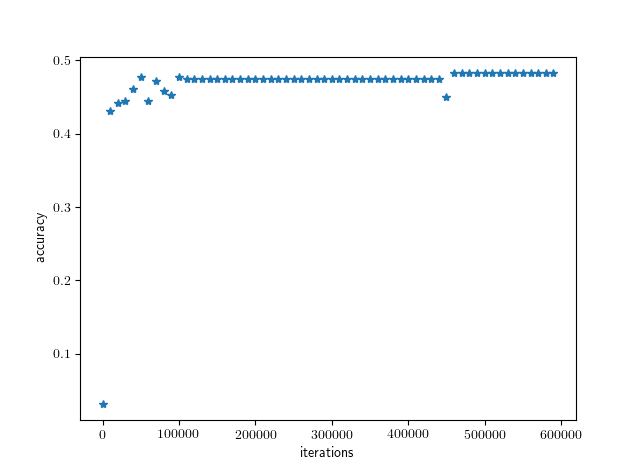
\includegraphics[width=\linewidth]{img/tests/lwf/40ppl/PCA_MLPk20h11}
\caption{10 hidden neurons, k = 15}
\end{subfigure}
\begin{subfigure}[b]{.45\linewidth}
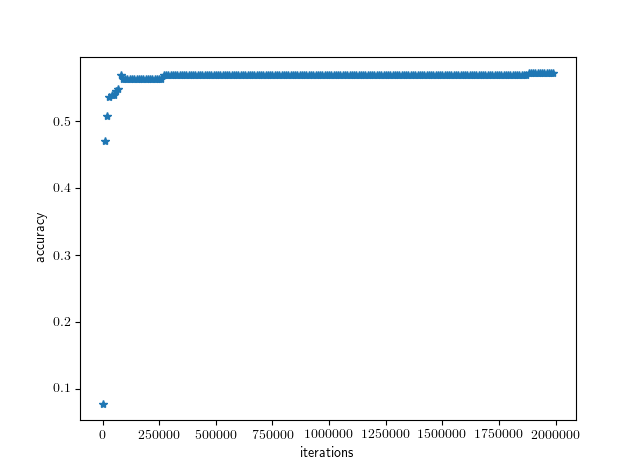
\includegraphics[width=\linewidth]{img/tests/lwf/40ppl/PCA_MLPk1520}
\caption{20 hidden neurons, k = 15}
\end{subfigure}


\begin{subfigure}[b]{.45\linewidth}
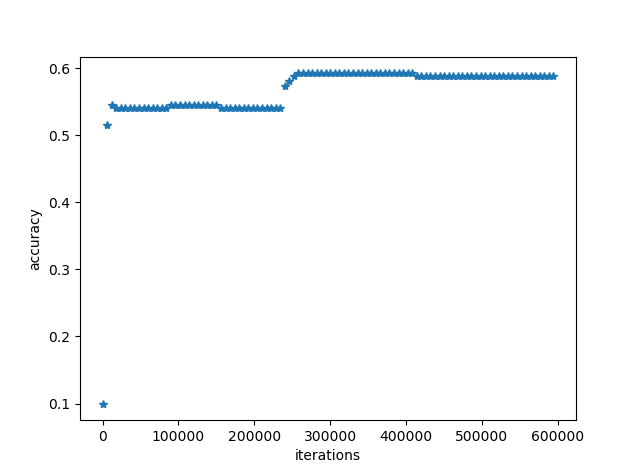
\includegraphics[width=\linewidth]{img/tests/lwf/40ppl/PCA_MLPk10h20}
\caption{10 hidden neurons, k = 10}
\end{subfigure}
\begin{subfigure}[b]{.45\linewidth}
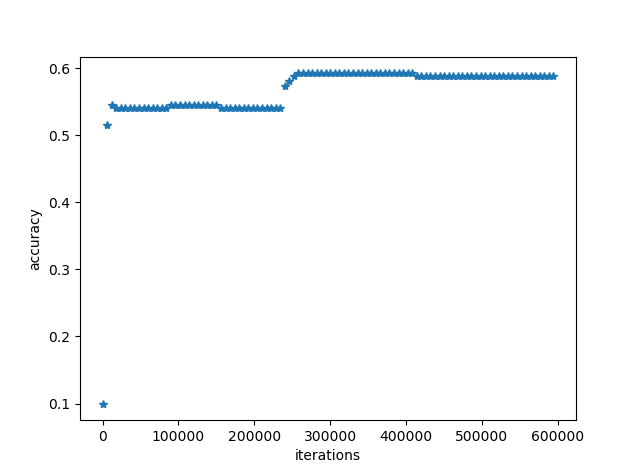
\includegraphics[width=\linewidth]{img/tests/lwf/40ppl/PCA_MLPk10h20.png}
\caption{20 hidden neurons, k = 10}
\end{subfigure}
\caption{Training accuracy for different amount of hidden neurons and eigenfaces}
\end{figure}

During experiment it was noticeable that the training accuracy grows with increasing the amount of hidden neurons. However, the time to train the network also grows and sometimes it was too long to see the performance:

\begin{figure}[H]
\centering
\begin{subfigure}[b]{.45\linewidth}
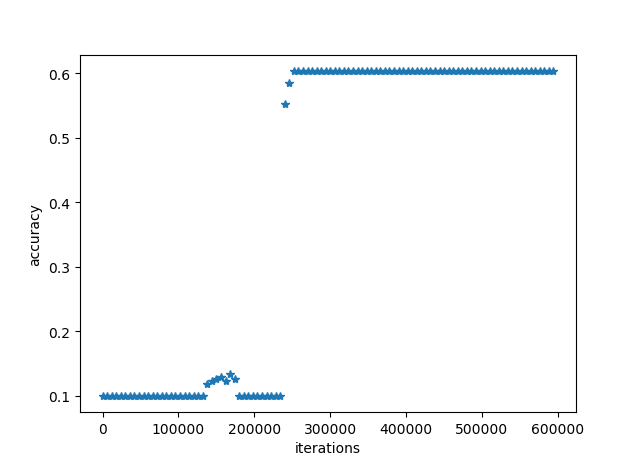
\includegraphics[width=\linewidth]{img/tests/lwf/40ppl/PCA_MLPk15h25}
\caption{25 hidden neurons, k = 15}
\end{subfigure}
\begin{subfigure}[b]{.45\linewidth}
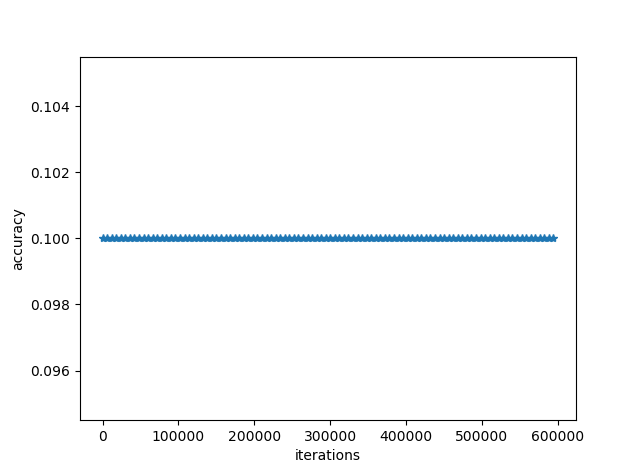
\includegraphics[width=\linewidth]{img/tests/lwf/40ppl/PCA_MLPk15h35.png}
\caption{30 hidden neurons, k = 15}
\end{subfigure}
\caption{Training accuracy for different amount of hidden neurons}
\end{figure}


After several experiments the best result was achieved with the model trained with 13 eigenfaces and 20 hidden neurons.


\begin{figure}[H]
\centering
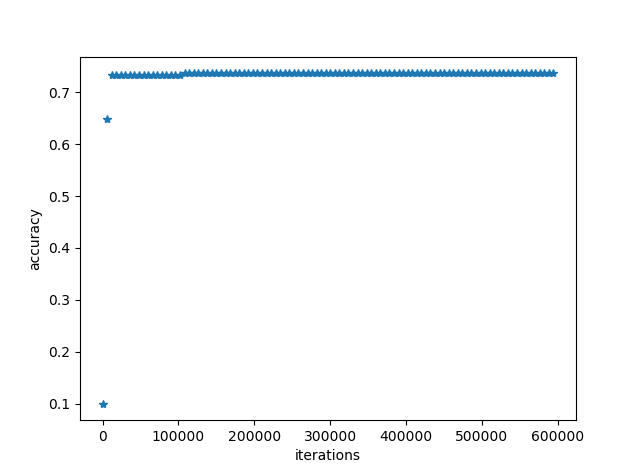
\includegraphics[scale=0.5]{img/tests/lwf/40ppl/PCAk15h20.png}
\caption{20 hidden neurons, k = 13}
\end{figure} 

The obtained recognition rate was 56.6\%, which is much better then PCA result but still not acceptable for facial recognition system. However, taking into consideration the quality and variety of images used for these tests, the result is better than expected.


\subsection{Two hidden layers}

Further experiments were performed on network topology presented on figure( ???). The goal is to check if additional hidden layer improves the network performance.

\begin{figure}[!h]
\centering
\begin{tikzpicture}[
           > = Stealth, semithick,
plain/.style = {draw=none, fill=none, yshift=11mm,
                text width=7ex,  align=center},% for text in images, 
   ec/.style = {draw=none},% for emty cells
  net/.style = {% for matrix style
    matrix of nodes,
    nodes={circle, draw, semithick, minimum size=12mm, inner sep=0mm},% circles in image
    nodes in empty cells,% for not used cells in matrix
  column sep = 16mm, % distance between columns in matrix 
     row sep = -3mm  % distance between rows in matrix
            },
]
\matrix[net] (m)% m is matrix name, it is used for names of cell: firs has name m-1-1
                % in empty space between ampersands will show circles: 
                % i.e.: nodes of the neural network
{
|[plain]| $Input$ & |[plain]| $Hidden_1$ &  |[plain]| $Hidden_2$& |[plain]| $Output$ \\
|[ec]|                &                         &                           & |[ec]|                  \\
                      & |[ec]|                  & |[ec]|                    & |[ec]|                  \\
|[ec]|                &                         &                           &                         \\
                      & |[ec]|                  & |[ec]|                   &  |[ec]|                  \\
|[ec]|                &                         &                           &                         \\
                      & |[ec]|                  & |[ec]|                    & |[ec]|                  \\
|[ec]|                &                         &                           & |[ec]|                  \\
};
\% inputs
\foreach \in [count=\ir from 1] in {3,5,7}
\draw[<-] (m-\in-1.west) -- node[above] {} +(-12mm,0);
% connections between nodes in the first and second layer
\foreach \j in {3,5,7}
{
\foreach \k in {2,4,6,8} \draw[->] (m-\j-1) -- (m-\k-2);
}
% connections between nodes in the second and third layer
\foreach \j in {2,4,6,8}
{
\foreach \k in {2,4,6, 8} \draw[->] (m-\j-2) -- (m-\k-3);
}

\foreach \j in {2,4,6,8}
{
\foreach \k in {4,6} \draw[->] (m-\j-3) -- (m-\k-4);
}
% output
% output
\draw[->] (m-4-4.east) -- node[above] {} +(12mm,0);
\draw[->] (m-6-4.east) -- node[above] {} +(12mm,0);
\end{tikzpicture}
\caption{Neural Network with two hidden layers}
\end{figure}

The first tests were ran with following parameters:

\begin{itemize}
\itemsep0em
\item number of hidden layers = 2
\item initial weights chosen randomly in a range [0:1]
\item sigmoid activation function
\item learning parameter = 0.2
\item number of eigenfaces = 15
\end{itemize}

Results are presented on figure( ??)


\begin{figure}[H]
\centering
\begin{subfigure}[b]{.45\linewidth}
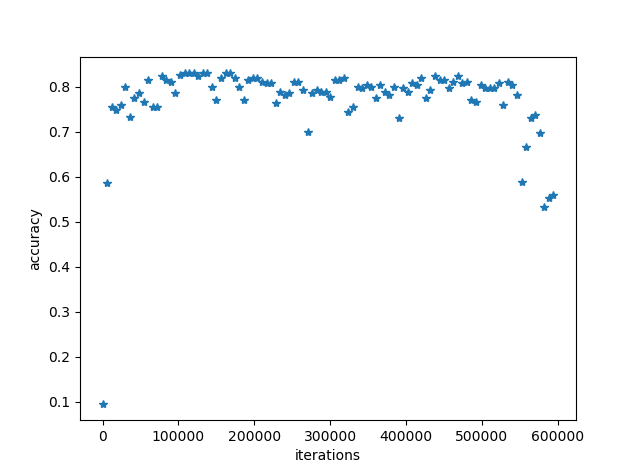
\includegraphics[width=\linewidth]{img/tests/lwf/40ppl/h2/PCA_MLP15_10_102.png}
\end{subfigure}
\begin{subfigure}[b]{.45\linewidth}
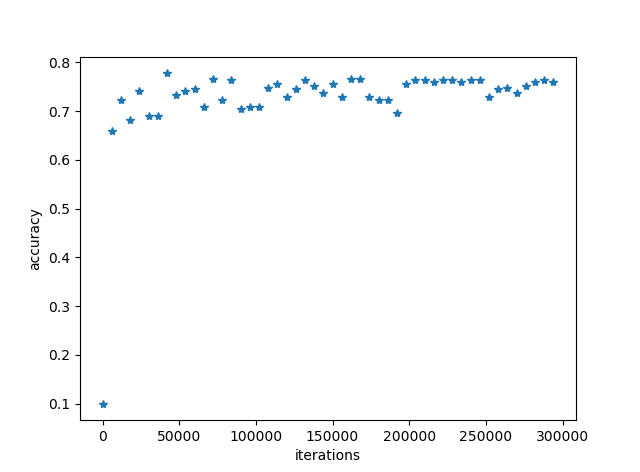
\includegraphics[width=\linewidth]{img/tests/lwf/40ppl/h2/PCA_MLP15_10_103.png}
\end{subfigure}
\caption{10 hidden neurons in each hidden layers, learning rate = 0.2}
\end{figure}

The system seemed to be very unstable. The learning rate was reduced to $0.05$ with the following results:

\begin{figure}[H]
\centering
\begin{subfigure}[b]{.45\linewidth}
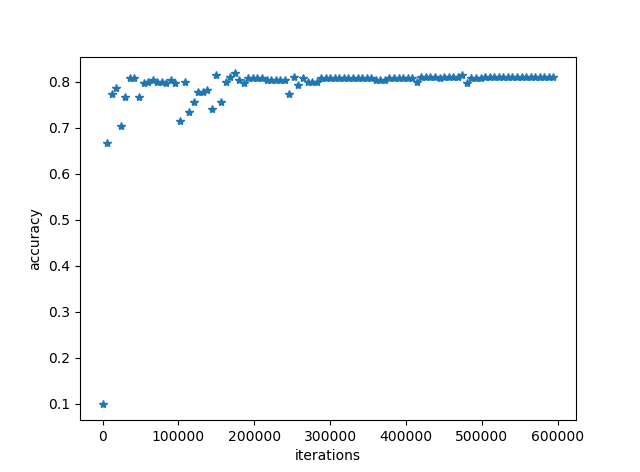
\includegraphics[width=\linewidth]{img/tests/lwf/40ppl/h2/PCA_MLP15_10_10.png}
\end{subfigure}
\begin{subfigure}[b]{.45\linewidth}
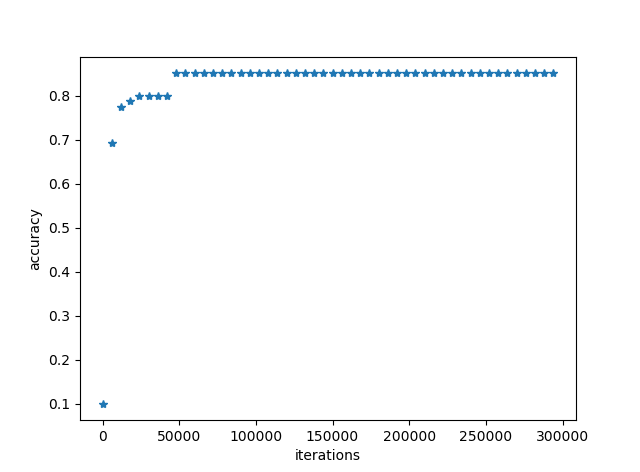
\includegraphics[width=\linewidth]{img/tests/lwf/40ppl/h2/PCA_MLP15_10_101.png}
\end{subfigure}
\caption{10 hidden neurons in each hidden layers, learning rate = 0.05}
\end{figure}


Better results were obtained with slightly bigger number of neurons in the second hidden layer. 

The network with following parameters gave the best training results:

\begin{itemize}
\itemsep0em
\item number of hidden layers = 2
\item 10 neurons in first hidden layer
\item 15 neurons in second hidden layer
\item initial weights chosen randomly in a range [0:1]
\item sigmoid activation function
\item learning parameter = 0.05
\item number of eigenfaces = 15
\end{itemize}


\begin{figure}[H]
\centering
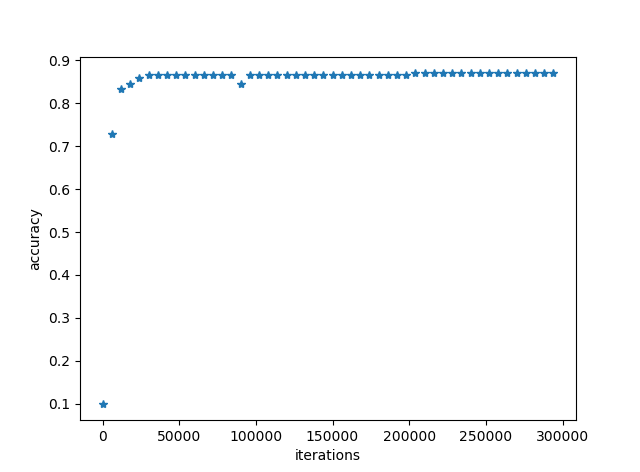
\includegraphics[scale=0.5]{img/tests/lwf/40ppl/h2/PCA_MLP15_10_104_best.png}
\caption{10 neurons in first hidden layer, 15 in the second hidden layer}
\end{figure}


The obtained recognition rate is 73.3\%. 

The presented results varies significantly on the values of initial weights and since the weights were chosen randomly it was a matter of error and trial to find an appropriate network configuration and train the network properly. It is possible that this score still can be improved. 



\chapter{Convolutional Neural Networks}
Convolutional Neural Network is a class of deep, feed-forward neural network, that can be successfully applied to systems with high dimensional input such as images.

It is a pattern recognition mechanisms that is inspired by the way in which mammals visually perceive the world around them using a layered architecture of neurons in the brain. 

Convolutional Neural Networks leverage three ideas:
\begin{enumerate}
\itemsep0em 
\item local connectivity
\item parameter sharing
\item pooling hidden units
\end{enumerate}

CNNs exploit spatially-local correlation by enforcing a local connectivity pattern between neurons of adjacent layers. In other words, each unit in the convolutional hidden layer is not connected with all units in a previous layer, instead it is connected to a subset of units from a previous layer. This approach helps to solve the problem of unmanageable number of parameters. 


The primary purpose of convolution in case of a CNNs is to extract features from the input image. In convolutional layer, the set of filters (typically square matrices with random values) is generated. 

Each filter is replicated across the entire visual field. These replicated units share the same parameterization (weight vector and bias) and form a feature (activation) map. Activation maps indicate ‘activated’ regions, i.e. regions where features specific to the filter have been detected in the input. 

Computation of those feature maps corresponds to computation of discrete convolution of a $i_{th}$ channel of input and filter matrix $W \in \Re^{2h_{1}+1 \times 2h_{2}+1}$. 

The convolution operation is given by
\begin{equation}
(X \ast W)_{r,s} = \sum_{u=-h_{1}}^{h_{1}}\sum_{v=-h_{2}}^{h_{2}} W_{u,v}X_{r+u,s+v}
\end{equation}

\begin{equation}
W =
\left[
\begin{matrix}
w_{-h_{1},-h_{2}} & \cdots & w_{-h_{1},h_{2}}  \\
\vdots & w_{0,0}& \vdots\\
w_{h_{1},-h_{2}} & \cdots & w_{h_{1},h_{2}} 
\end{matrix}
\right]
\end{equation}

The behaviour of this operation towards the borders of the image is handle by 0-padding if needed. 

The $i_th$ feature map in layer $l$ is computer as  

\begin{equation}
z_{i}^{(l)} = \sum_{j=1}^{m} K_{i,j}^{(l)} \ast Y_{j}^{l-1}
\end{equation}
where $m$ is the size of the $l$ layer input.

The output of the layer l, denoted $Y_{i}^{(l)}$ is given by

\begin{equation}
Y_{i}^{(l)} = f\Big(z_{i}^{(l)}\Big)
\end{equation}
where $f$ is an activation function.

The values of the filter matrix change with each learning iteration over the training set, indicating that the network is learning to identify which regions are of significance for extracting features from the data. 

Another important concept of CNNs is max-pooling, which is a form of non-linear down-sampling. Max-pooling partitions the input image into a set of non- overlapping rectangles and, for each such subregion, outputs the maximum value.
Max-pooling is useful in vision for two reasons: 

\begin{itemize}
\itemsep0em 
\item By eliminating non-maximal values, it reduces computation for upper layers.
\item It provides a form of translation invariance.
\end{itemize}

Since it provides additional robustness to position, max-pooling is a “smart” way of reducing the dimensionality.
\\\\\\\\
After a sequence of those operation the output is flattened and applied to the fully connected layer.
At the very end of the network the output is squashed with the softmax layer, so that each element in the output vector corresponds to the probability value for each class.

\begin{equation}
\sigma(o_{j}) = \frac{e^{o_{j}}}{\sum_{k=1}^{K} e^{o_{k}}}
\end{equation}

where $K$ is the number of classes and $o_{j}$ is the $j_{th}$ value of the output vector.

The whole process is presented in the figure (??) 

\begin{figure}[H]
\centering
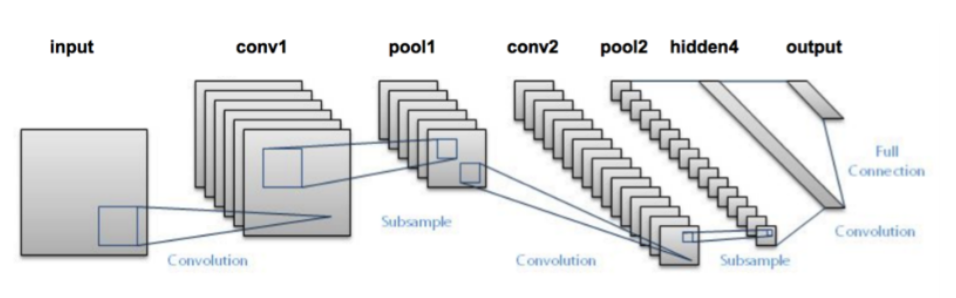
\includegraphics[scale=0.7]{img/proces.png}
\caption{A typical convolutional neural network for face recognition}
\end{figure}

The algorithm is trained with backpropagation. 
The backpropagation algoritihm for convolutional neural networks is slightly more complicated than the one for Multilayered Perception. The general idea is exactly the same, but in CNN we have to face with backpropagation through flatenning, maxpooling and convolution, which requires more effort in practice. 

The first step, as in MLP, is to calculate the error between predicted and expected class probabilities. To do that we calculate the cross entropy error.
Cross entropy measure is widely used when the network output represents the class probabilities. Thus it is used as a loss function in neural networks which have softmax activations in the output layer.


The softmax activation of the ith output unit is: 

\begin{equation}
o_{i} = \frac{e^{s_{i}}}{\sum_{k=1}^{K} e^{s_{k}}}
\end{equation}

where $K$ is the number of classes and $s_{i}$ is the $i_{th}$ value of the last dense layer output vector.

The cross entropy function for multi-class output is given by:

\begin{equation}
E(o, o') = -\sum_{i=1}^K o'_{i} \ln(o_{i})\end{equation} 

\begin{equation}
E = -\sum_{i=1}^K o'_{i} \ln(o_{i})
\end{equation} 

Computing the gradient yields
\begin{equation}
\frac{\partial E}{\partial o_{i}} = -\frac{o'_{i}}{o_{i}}
\end{equation}

\begin{equation}
\begin{split}
\frac{\partial o_i}{\partial s_k}  & = \left\{ \begin{array}{ll}
\frac{e^{s_{i}}}{\sum_{j=1}^{K} e^{s_{j}}} - \Big(\frac{e^{s_{i}}}{\sum_{j=1}^{K} e^{s_{j}}}\Big)^2 & \textrm{$i\neq k$}\\
-\frac{e^{s_{i}} e^{s_{k}}}{(\sum_{j=1}^{K}e^{s_{j}})^2} & \textrm{$i=k$}
\end{array} \right. \\
& = \left\{ \begin{array}{ll}
o_i (1-o_i)& \textrm{$i\neq k$}\\
-o_i o_k & \textrm{$i=k$}
\end{array} \right.
\end{split}
\end{equation}

\begin{equation} 
\begin{split}
\frac{\partial E}{\partial s_i} & = \sum_k^{K} \frac{\partial E}{\partial o_{k}} \frac{\partial o_{k}}{\partial s_{i}} \\
 & = \frac{\partial E}{\partial o_{i}} \frac{\partial o_{i}}{\partial s_{i}} - \sum_{k \neq i} \frac{\partial E}{\partial o_{k}}\frac{\partial o_{k}}{\partial s_{i}}\\
& = o'_{i} (1- o_{i}) + \sum_{k \neq i} o'_{k}o_{i}\\
& = o't_{i} + o_{i} \sum_{k} o'_{k} \\
& = o_{i} - o'_{i}
\end{split}
\end{equation}

The gradient for weight in the last dense layer can be computed as follows:

\begin{equation}
\begin{split}
\frac{\partial E}{\partial w_{ji}} & = \sum_{i}\frac{\partial E}{\partial s_{i}} \frac{\partial s_{i}}{\partial w_{ji}}\\
& = (o_{i} - o'_{i})h_{j}
\end{split}
\end{equation}

where $h_{j}$ is the output of the first dense layer in the network and $w_{ij}$ is the weight connecting the units from second dense layer to the output layer.

The error is backpropagated further as described in chapter 4.3 (??).

The next step is to perform the reversed flatten layer, so that the error can be backpropagated further to maxpooling layer. Backpropagating through maxpooling layer implements the idea that the gradient from the flatten layer is passed back to only that neurons which achieved the maximum value in forward pass during maxpooling computation. All other neurons get zero gradient.

The gradient prepared in such a way is ready to be backpropagated through convolutional layers.
The backpropagation for convolutional layer can be applied as described in chapter 4, however equation 4.12 changes to:

\begin{equation}
\Delta w_{ij} = \lambda z_{j}^{(l-1)} \sum_{k=1}^{m^{(l)}}\delta_k^{(l)}
\end{equation}

As in every other Artificial Neural Network training process can be decomposed in the following steps:

\begin{enumerate}
\itemsep0em 
\item Feed-forward pass
\item Backpropagation of each layer
\item Weight updates
\end{enumerate}

The algorithm is stopped when the value of the error function is sufficiently small.

DeepFace [Taigman et al., 2014] and FaceNet [Schroff, Kalenichenko, and Philbin, 2015] are two of the most successful applications of CNNs in the Face Recognition  problem. These two have provided state-of-art results in recent years, with the best results being obtained by the second one.

\section{Implementation and test results}

The Convolutional Neural Network may differ in number of layers and their connections. The one that was implemented has the following architecture:

\begin{python}
    def forward_pass(self, X):
        h = self.relu(self.cnn_layer(X, layer_i=0, border_mode="full"))
        h = self.relu(self.cnn_layer(h, layer_i=1, border_mode="valid"))
        h = self.maxpooling_layer(h)
        h = self.relu(self.cnn_layer(h, layer_i=3, border_mode="valid"))
        h = self.maxpooling_layer(h)
        h = self.flatten_layer(h)
        h = self.relu(self.dense_layer(h, layer_i=6))
        h = self.dense_layer(h, layer_i=7)
        h = self.softmax_layer2D(h)
        max_i = self.classify(h)
      	return max_i[0]
\end{python}

The first two and the 4th layer in the network performs the convolutional operation followed by activation function RELU.

The input to the network is an image, that can be treated as matrix with three dimensions, each corresponding to every color channel (RGB). In this case every image has the same width and height $k$ equal to 76 pixels. 

\begin{equation}
R =
\left[
\begin{matrix}
r_{11} & r_{21} & \cdots & \cdots & r_{k1}\\
r_{12} & r_{22} & \cdots & \cdots & r_{k2}\\
r_{13} & r_{23} & \cdots & \cdots & r_{k3}\\
r_{14} & r_{24} & \cdots & \cdots & r_{k4}\\
\cdots & \cdots & \cdots & \cdots & \cdots\\
\cdots & \cdots & \cdots & \cdots & \cdots\\
r_{1k} & r_{2k} & \cdots & \cdots & r_{kk}
\end{matrix}
\right]
G =
\left[
\begin{matrix}
g_{11} & g_{21} & \cdots & \cdots & g_{k1}\\
g_{12} & g_{22} & \cdots & \cdots & g_{k2}\\
g_{13} & g_{23} & \cdots & \cdots & g_{k3}\\
g_{14} & g_{24} & \cdots & \cdots & g_{k4}\\
\cdots & \cdots & \cdots & \cdots & \cdots\\
\cdots & \cdots & \cdots & \cdots & \cdots\\
g_{1k} & g_{2k} & \cdots & \cdots & g_{kk}
\end{matrix}
\right]
B =
\left[
\begin{matrix}
b_{11} & b_{21} & \cdots & \cdots & b_{k1}\\
b_{12} & b_{22} & \cdots & \cdots & b_{k2}\\
b_{13} & b_{23} & \cdots & \cdots & b_{k3}\\
b_{14} & b_{24} & \cdots & \cdots & b_{k4}\\
\cdots & \cdots & \cdots & \cdots & \cdots\\
\cdots & \cdots & \cdots & \cdots & \cdots\\
b_{1k} & b_{2k} & \cdots & \cdots & b_{kk}
\end{matrix}
\right]
\end{equation}

In convolutional layer each of those matrices were convolved with each of 32 randomly chosen filters. The convolutional layer has an additional parameter \textit{border mode}, which can be set to either \textit{full} or \textit{valid}, which defines if the convolution operation involves padding around the input (valid border mode sets padding to $0$).
The convolution across each channel is summed up. As a result first two layers we obtain a matrix with dimensions = $(1, 32, 76, 76)$.


The 3rd and the 5th layer are maxpooling layers, which purpose is to reduce the dimensionality of the data. No activation function is applied. The 3rd and 5th output matrix dimensions are accordingly: $(1, 32, 38, 38)$ and $(1, 32, 18, 18)$.

One of the last stages of a convolutional neural network (CNN) is a dense layer. It's just a simple MLP layer, as described in chapter(??). It requires the one-dimensional input - the output of convolutional layers has to be converted into a 1D feature vector. This operation is called flattening and is performed with the flatten layer. 
After flattening the data we obtain a vector with $10368 (18*18*32)$ elements. The MLP layer used in this example has one hidden layer with $6000$ units. The output layer consist of number of units equals to the number of classes (amount of people in the database) - in our case $20$. 

The last part of the network is a softmax layer, which allows us to calculate the probability value for each class.

The above construction allows to classify an image only if the filter parameters and dense layer parameters are set correctly. The choice of those coefficients is made randomly and they are trained with backpropagation algorithm. 

During the algorithm implementation it turned out that training the entire network on a reasonably sized dataset would be unfeasible on a personal laptop. Even though the dimensionality reduction (maxpooling)is applied, the total number of parameters that need to be trained is equal to ~ $1,25*10^9$. 

According to the convolutional networks theory we know that the goal of the lower layers is to identify lower-level features such as colors, shapes or textures, and only the top layers distinguish the specific, higher-level features of each class. Based on this idea, instead of training the whole convolutional network, we can take an existing convolutional network model and train the last layer of the network so that it can recognize the given data. 

The first experiment was performed with Google Inception-v3 model. The Inception v3 model has nearly 25 million parameters and uses 5 billion multiply-add operations for classifying a single image.

\begin{figure}[H]
\centering
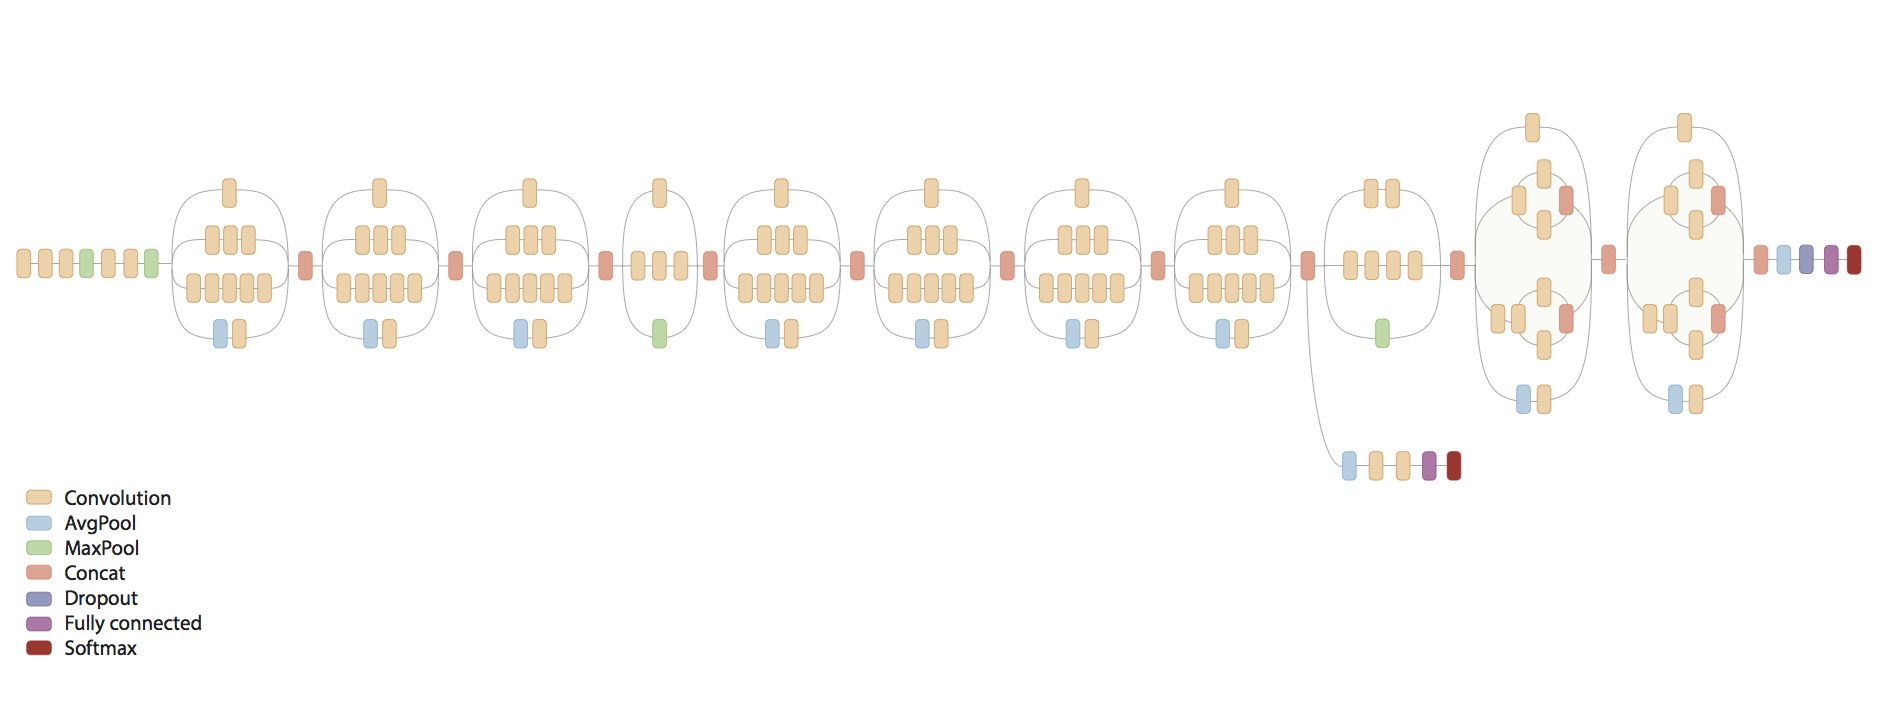
\includegraphics[scale=0.5]{img/inception_v3_architecture.png}
\caption{Google Inception v3 model architecture}
\end{figure}

This model structure is much more complicated than the general convolutional network architecture. Instead of applying all convolutional, maxpooling and dense layers one by one, some of the layers consist of the composition of those operation. The model was trained on ImageNet database with 1000 image categories and turns out to outperform the human recognition abilities. The goal of this experiment is to find out how good this model can be adjusted to recognize human faces, taking into account that there was no facial images in its training data set. 

The tensofflow library provides the function that returns  the outputs from a different layers. We take the last layer with 2048 neurons and connect it to the fully connected layer, creating a new output with amount of neurons corresponding to the amount of individuals in the dataset. To train only a single layer, we specify the list of trainable variables in the training operation. The network will train only the parameters that connects the 2048 inception neurons with 10 output neurons of our network. At the end the softmax activation function is applied in order to calculate probabilities for each class.


\section{Test results}

Algorithm was implemented in Python 3.4 with usage of numpy and tensorflow libraries. 

The test was performed on 10 individuals with the biggest amount of images from Labeled Faces in Wild database. 

\begin{table}[H]
	\centering
	\caption{List of individuals taken for testing the algorithm}
    \begin{tabular}{ | l | l |}
    \hline
    \rowcolor{lightgray}
    Name &  Number of pictures \\ \hline
	George W. Bush & $100$\\  \hline  
	Colin Powell & $100$ \\ \hline    
	Tony Blair & $100$\\\hline
    Donald Rumsfeld  & $100$ \\ \hline
    Gerhard Schroeder  & $100$\\ \hline
    Ariel Sharon &  $77$  \\ \hline
	Hugo Chavez & $71$\\\hline
    Junichiro Koizumi  & $60$\\\hline    
    Jean Chretien  & $55$\\\hline
    John Ashcroft  & $53$\\
    \hline
    \end{tabular}
\end{table}

Data was randomly separated into three sets:
\begin{itemize}
\itemsep0em 
\item 75\% training set
\item 5\% validation set
\item 20\% testing set
\end{itemize}

The algorithm implements early stopping approach. It requires periodically testing the network on a validation set to obtain the score on the cost function (average cross entropy). If the loss does not decrease for a specified number of iterations, training is interrupted. It prevents the network from overfitting. 

The test results visualization were generated by tensorboard module (from tensorflow library).

\begin{figure}[H]
\centering
\includegraphics[scale=0.5]{img/train_acc.png}
\caption{Training accuracy}
\end{figure}

\begin{figure}[H]
\centering
\includegraphics[scale=0.5]{img/valid_loss.png}
\caption{Validation loss}
\end{figure}

Taking into account that these results were obtained via training only last layer of the network, we can consider them better than expected. The training accuracy reached ~80\%.

The recognition rate obtained from testing data set was 83,8\%.

The Chicago Face Database was not tested due to not enough training data that is required for this algorithm. 

\chapter{Support Vectors Machine}

\section{Algorithm background}

SVM belong to the class of maximum margin classifiers. They perform pattern recognition between two classes by finding a decision surface that has maximum distance to the closest points in the training set which are termed support vectors.

We start with a training set of points $x_{i} \in R$, $i = 1,2 ... N$ where each point $x_{i}$ belongs to one of two classes identified by the label $y \in { {1,-1} }$ Assuming that data is linearly separable, the goal of SVM is to separate the two classes by a hyperplane.

\begin{figure}[H]
\centering
\includegraphics[scale=0.5]{img/svm/linear.png}
\caption{Linearly separable dataset and its hyperplane}
\end{figure} 

The hyperplane is a set of points satisfying equation 4.1

\begin{equation}
f(x) = w^T x + b = 0
\end{equation}

The vector $w$ is known as the weight vector, and $b$ is called the bias. 
Suppose the weight vector can be expressed as a linear combination of the training examples, i.e.

\begin{equation}
w = \sum_{i=1}^{N} \alpha_{i}x_{i}
\end{equation}

Then:

\begin{equation}
f(x) = \sum_{i=1}^{N} \alpha_{i}x_{i}^T x + b
\end{equation}

The representation in terms of the variables $\alpha_{i}$ is known as the dual representation of the decision boundary.

The hyperplane divides the space into two: the sign of the discriminant function  denotes the side of the
hyperplane a point is on.

\subsection{The geometric margin}
For a given hyperlane we denote by $x_{+}$ the closest point to the hyperpalne among the positive examples and by $x_{-}$ the closest point to the hyperpalne among the negative examples. These points are commonly called support vectors.
The margin of a hyperplane f can be described as:

\begin{equation}
m(f) = \frac{1}{2}\uvec{w}^{T}(x_{+}-x_{-}) 
\end{equation}

where $\uvec{w}$ is a unit vector in the direction of w. We assume that $x_{+}$ and $x_{-}$ are equidistant from
the hyperplane:

\begin{equation}
f(x_{+}) = w^Tx_{+} + b = a
f(x_{-}) = w^Tx_{-} + b = -a
\end{equation}

where $a>0$

Adding the two equations and dividing by $||w||$ we can describe the geometric margin as:
\begin{equation}
m(f) = \frac{1}{||w||}
\end{equation}

The purpose of the algorithm is to maximize the geometric margin. This optimization problem can be also seen as minimizing $||w||^2$

\begin{equation}
\begin{multlined}
\min_{w,b} \frac{1}{2}||w||^2 \\
s.t. \forall i, y_{i}(w^Tx_{i} + b) \geq 1
\end{multlined}
\end{equation}

The constraints in this formulation ensure that the maximum margin classifier classifies each example correctly. However, in our optimization problem we want to introduce some kind of "penalty" for data misclassification. This can be done with changing our optimization problem to so-called soft-margin SVM:

\begin{equation}
\begin{multlined}
\min_{w,b} \frac{1}{2}||w||^2 + C \sum_{i=1}^{N} \xi_{i}\\
s.t. \forall i, y_{i}(w^Tx_{i} + b) \geq 1 - \xi_{i}
\end{multlined}
\end{equation}

where $\xi_{i}\geq 0$ are so-called \textit{slack variables} that allow an example to be in the margin ($0\leq \xi_{i}\geq 1$, also called a margin error) or to be misclassified ($\xi_{i} > 1$).

\begin{figure}[H]
\centering
\includegraphics[scale=0.5]{img/svm/ksi.png}
\caption{Illustration of $\xi$ value}
\end{figure} 

The parameter C is called \textit{slack penalty} and is one of the SVM "tuning" parameters.

The solution to this optimization problem can be solved using Lagrange duality principle.

Classification of a new data point is performed by computing the  (?) equation with previously optimized parameters.

\begin{equation}
h_{w,b}(x) = g(w^T x + b)
\end{equation}

where $w$ and $b$ are coefficients of the hyperplane trained by SVM algorithm and $g(z)=1$ if $z\geq0$, and $g(z)=-1$ otherwise.


\subsection{Non linear separable dataset}

The described approach works only for linearly separable data set. Nevertheless, in many applications a non-linear classifier is required. Linear classifiers have several advantages, one of them being that they often have simple training algorithms. 
This begs the question: Can we extend the entire linear-classifier construction to generate non-linear decision boundaries? 

\begin{figure}[H]
\centering
\includegraphics[scale=0.5]{img/svm/nonlinear.png}
\caption{Nonlinearly separable dataset and its hyperplane}
\end{figure} 

The solution to this problem is to map our data from
the input space X to a feature space F using a non-linear function $\phi : X \rightarrow F$, so that the entire construction can be extended to the case of nonlinear separating surfaces. 

Each point $x_{i}$ in the input data is mapped to a point $z = \phi(x)$ of a higher dimensional space, called the feature space.

Rather than applying SVMs using the original input attributes x, we learn the algorithm using new features $\phi(x)$ instead.

To map our training set into the higher dimensional space we choose the similarity 

For each $x_{i}$ we calculate the similarity value between this  and every other sample in the data set. The similarity function is also called a kernel.

\begin{equation}
\begin{multlined}
\\
f_{i1} = K(x_{i}, x_{1})\\
f_{i2} = K(x_{i}, x_{2})\\
\vdots\\
f_{iN} = K(x_{i}, x_{N})
\end{multlined}
\end{equation}

In the new high dimensional space each point $x_{i}$ is represented as a vector:

\begin{equation}
\vec{f_{i}} = [f_{i1}, f_{i2}, \cdots, f_{iN}]
\end{equation}

In the feature space, F expression 4.3 takes the form:

\begin{equation}
f(x) = \sum_{i=1}^{N} \alpha_{i}\phi(x_{i})^T \phi(x) + b
\end{equation}
The feature space F may be very high dimensional, hence computing the whole equation becomes computationally expensive unless the kernel function K, defined by equation( ??) can be computed efficiently.
\begin{equation}
K(x,z) = \phi(x)^T\phi(z)
\end{equation}

Using the kernel function the decision boundary function can be defined as: 

\begin{equation}
f(x) = \sum_{i=1}^{N} \alpha_{i}K(x, x_{i})+ b
\end{equation}

Two most widely used kernels are:
\begin{enumerate}
\itemsep0em 
\item Gaussian kernel
\begin{equation}
K(x,x_{i}) = exp(-\frac{||x-x_{i}||^2}{2\sigma^2})
\end{equation}
where $\sigma$ is a parameter that controls the width of Gaussian
\item Polynomial kernel 
\begin{equation}
K(x,x_{i}) = [(x \cdot x_{i} + 1]^d
\end{equation}
with degree d
\end{enumerate} 


\subsection{Multi-class classification problem}

There are two basic approaches for solving n-class problems with SVMs:
\begin{enumerate}
\itemsep0em 
\item one-vs-all approach - q SVMs are trained. Each of the SVMs separates a single class from all remaining classes.
\item pairwise approach - q(q-1)/2 SVMs are trained. Each SVM separates a pair of classes. The pairwise classifiers are arranged in trees, where each tree node represents an SVM. 
\end{enumerate}

\subsection{Face recognition}
The system has a linear SVM for every person in the database. Each SVM is trained to distinguish between all images of a single person and all other images. Given a set of q people and a set of q SVMs, each one associated to one person, it is relatively easy to perform recognition. Specifying the threshold, the distance between input and given SVM models are computed as follows:

\begin{equation}
d(x) = \frac{•\sum_{i=1}^l \alpha_{i}y_{i}x_{i} \cdot x + b}{||\sum_{i=1}^l\alpha_{i}y_{i}x_{i}||}
\end{equation}

We can notice that numerator is equal to right side of equation (12), hence the sign of $d$ is the classification result for x, and $||d||$ is the distance from x to the hyperplane.

The class label of input picture is computed as follows:

$y = \begin{cases} n$ if $d_{n}(x) > t \\$ not recognized if $d_{n}(x) \leq t \end{cases}$

where $d_n(x) = max ({d_{i}}_{i=1}^q)$

\section{Implementation and test results}

The SVM algorithm was implemented with Python 3.6.1 with usage of numpy, PIL and sklearn libraries. 

The first step in the algorithm is data preprocession. As in the Multilayered Perception approach, the images were preprocessed with PCA algorithm in order to reduce the dimensionality of input data, hence reducing the computational complexity of the algorithm. The algorithm is using one-vs-one approach.

The tests were performed on two different databases: 
\begin{itemize}
\itemsep0em 
\item Chicago Face Database - pictures captured in controlled environment
\item Labeled Faces in Wild database - pictures captured in uncontrolled environment, with various lightning conditions, pose, facial expression etc. 
\end{itemize}

The main goal of the experiments was to examine the influence of parameter $C$ and different kernels on accuracy of the algorithm.

\section{Tests on pictures captured in controlled environment}

The database was divided into training and testing samples. The training was performed using 3 pictures of the individual, one picture was used to test the trained model. 

\subsection{20 individuals}

The first experiment was performed on 20 individuals from CFD database. 
The Gaussian and Polynomial kernels were tested. 

The Gaussian kernel as a similarity function that measures the “distance” between a pair of examples, ($x_{i}$, $x_{j}$). The Gaussian kernel is also parameterized by a bandwidth parameter $\sigma$ (equation(???), which determines how fast the similarity metric decreases to 0 as the examples are further apart. 

The kernel function from equtaion (???) can be also interpreted as:

\begin{equation}
exp(-\gamma * ||x-x_{i}||^2)
\end{equation}

where:
\begin{equation}
\gamma = \frac{1}{2\sigma^2}
\end{equation}

The influence of $\gamma$ parameter on the gaussian kernel function can be visualized as presented on figure (??). (with the smallest value of $\gamma$ on the most left graph and the greatest on the right) 


\begin{figure}[H]
\centering
\includegraphics[scale=0.27]{img/svm/gaussian.png}
\caption{Gaussian kernel visualization}
\end{figure} 

The figure(??) presents the SVM training accuracy with varying $\gamma$ and C parameter:

\begin{figure}[H]
\centering
\includegraphics[scale=0.75]{img/svm/better_graphs/CFD_20i_rbf.png}
\caption{Training score with varying gamma and C parameter for 20 individuals}
\end{figure} 


The best score (~0.85) was obtained with several configurations of $C$ and $\gamma$ parameters. The further testing was performed with $C = 10^3$ and $\gamma = 10^-4$

In this configuration SVM algorithm reached 80\% of recognition rate on the testing samples.

The same experiment was performed with usage of polynomial kernel. 
The influence of polynomial degree was examined and is presented on figure (??).

\begin{figure}[H]
\centering
\includegraphics[scale=0.75]{img/svm/better_graphs/CFD_20i_poly.png}
\caption{Training score with varying polynomial degree and C parameter for 20 individuals}
\end{figure} 

On Figure(7.6 (??)) we can see that our data can be nicely separated with polynomial of second degree.  
The recognition rate was tested on SVM trained with $C = 10$ and the degree = 2.

Obtained result is ~70\%, which is 10 percentage points less than result of SVM trained with Gaussian kernel. 

\subsection{40 individuals}

The same test scenario was used to examine SVM on bigger amount of input data - 40 individuals.

The results are presented below.

\begin{figure}[H]
\centering
\includegraphics[scale=0.75]{img/svm/better_graphs/CFD_40i_rbf.png}
\caption{Training score with varying gamma and C parameter for 40 individuals}
\end{figure} 

The best score (~0.71) was obtained with several configurations of $C$ and $\gamma$ parameters. The further testing was performed with $C = 10^3$ and $\gamma = 10^-3$

In this configuration SVM algorithm reached 60\% of recognition rate on the testing samples.

The same experiment was performed with usage of polynomial kernel. 
The influence of polynomial degree was examined and is presented on figure (??).

\begin{figure}[H]
\centering
\includegraphics[scale=0.75]{img/svm/better_graphs/CFD_40i_poly.png}
\caption{Training score with varying polynomial degree and C parameter for 40 individuals}
\end{figure} 

The best score was obtained with degree = 2 and $C = 10^4$. With these parameters recognition rate reached ~52\%, which is still worse than SVM trained with Gaussian kernel.

\section{Tests on pictures captured in uncontrolled environment}

To test the algorithm the Labeled Faces in Wild database was used. The quality of images is much worse then in the previous examples, so the tests result are expected to be worse. 

Test was performed on 20 individuals with 30 pictures each. The training set for each person consists of 27 samples, 3 pictures were used to test the model. 

The results are presented below.

\begin{figure}[H]
\centering
\includegraphics[scale=0.75]{img/svm/better_graphs/lwf_rbf.png}
\caption{Training score with varying gamma and C parameter for 20 individuals}
\end{figure} 

The best training score ($~0.278$) was obtained with with $C = 10$ and $\gamma = 0.01$
In this configuration SVM algorithm reached 26,6\% of recognition rate on the testing samples.


The same experiment was performed with usage of polynomial kernel. 
The influence of polynomial degree was examined and is presented on figure (???).

\begin{figure}[H]
\centering
\includegraphics[scale=0.75]{img/svm/better_graphs/lwf_poly.png}
\caption{Training score with varying polynomial degree and C parameter for 20 individuals}
\end{figure} 

In this case, SVM obtained best results with third polynomial degree and $C = 10$. The obtained recognition rate was ~20\%.


\section{SVM summary}

To compare obtained results a tabular summary of the recognition rate for SVM algorithm with different kernels on each database is presented (Table 7.1).

\begin{table}[H]
	\centering
	\caption{A tabular summary of the recognition rate for SVM algorithm with different kernels on each database}
    \begin{tabular}{ | l | l | l | l |}
    \hline
    \rowcolor{lightgray}
    Database &  Gaussian kernel & Polynomial kernel\\ \hline
    CFD 20&  80\%  & 70\%\\ \hline
	CFD 40& $60\%$ & $52\%$ \\ \hline
    LFW & $26.6\%$ & $20\%$ \\ \hline
    \end{tabular}
\end{table}

From these tests we can conclude that the gaussian kernel allows us to obtain better results for every database. As expected, the results are significantly better for pictures captured in controlled environment and small amount of data. Even though SVM has an advantage of small computing time, the results do not meet the expectations of good facial recognition system. 


\chapter{Summary}

\begin{table}[H]
	\centering
	\caption{A tabular summary of the recognition rate for each algorithm}
    \begin{tabular}{ | l | l | l | l | l |}
    \hline
    \rowcolor{lightgray}
    Algorithm &  CFD 20 & CFD 40 & LFW 20 \\ \hline
    PCA &  $114$  & $173$ & $10$\\ \hline
	PCA-MLP & $70\%$ & $43.5\%$ & $10$ \\ \hline
    SVM & $76.5\%$ & $50\%$ & $10$ \\ \hline
    CNN & $76.5\%$ & $50\%$ & $10$ \\
    \hline
    \end{tabular}
\end{table}

\begin{table}[H]
	\centering
	\caption{A tabular summary of the execution time for each algorithm}
    \begin{tabular}{ | l | l | l | l | l |}
    \hline
    \rowcolor{lightgray}
    Algorithm &  CFD 20 & CFD 40 & LFW \\ \hline
    PCA &  $114$  & $173$ & $10$ \\ \hline
	PCA-MLP & $70\%$ & $43.5\%$ & $10$ \\ \hline
    SVM & $76.5\%$ & $50\%$ & $10$\\ \hline
    CNN & $76.5\%$ & $50\%$ & $10$\\
    \hline
    \end{tabular}
\end{table}


% itd.
% \appendix
% \include{dodatekA}
% \include{dodatekB}
% itd.

\bibliographystyle{alpha}
\bibliography{bibliografia}
%\begin{thebibliography}{1}
%
%\bibitem{Dil00}
%A.~Diller.
%\newblock {\em LaTeX wiersz po wierszu}.
%\newblock Wydawnictwo Helion, Gliwice, 2000.
%
%\bibitem{Lam92}
%L.~Lamport.
%\newblock {\em LaTeX system przygotowywania dokumentów}.
%\newblock Wydawnictwo Ariel, Krakow, 1992.
%
%\bibitem{Alvis2011}
%M.~Szpyrka.
%\newblock {\em {On Line Alvis Manual}}.
%\newblock AGH University of Science and Technology, 2011.cccccc
%\newblock \\\texttt{http://fm.ia.agh.edu.pl/alvis:manual}.
%
%\end{thebibliography}

\end{document}
